\documentclass[aspectratio=169]{beamer}

\usetheme[progressbar=frametitle]{metropolis}
\usepackage{appendixnumberbeamer}

\usepackage{booktabs}
\usepackage[scale=2]{ccicons}

\usepackage{pgfplots}
\usepgfplotslibrary{dateplot}

\usepackage{xspace}
\newcommand{\themename}{\textbf{\textsc{metropolis}}\xspace}

\title{Nonparametric Estimation of Matching Efficiency and Mismatch in Labor Markets via Public Employment Security Offices in Japan, 1972-2024}
\date{2024/7/9 Hitotsubashi U}
\subtitle{\textcolor{blue}{Preliminary}}
% \date{\today}

\author{Suguru Oani\\ University of Tokyo Market Design Center (UTMD)}
% \institute{}
%\date{\today}
% \titlegraphic{\hfill\includegraphics[height=1.5cm]{logo.pdf}}

\begin{document}

\maketitle

\section{Introduction}
\begin{frame}{Market Tightness \& Hires -> Research Question}
\begin{figure}[!ht]
  \begin{center}
  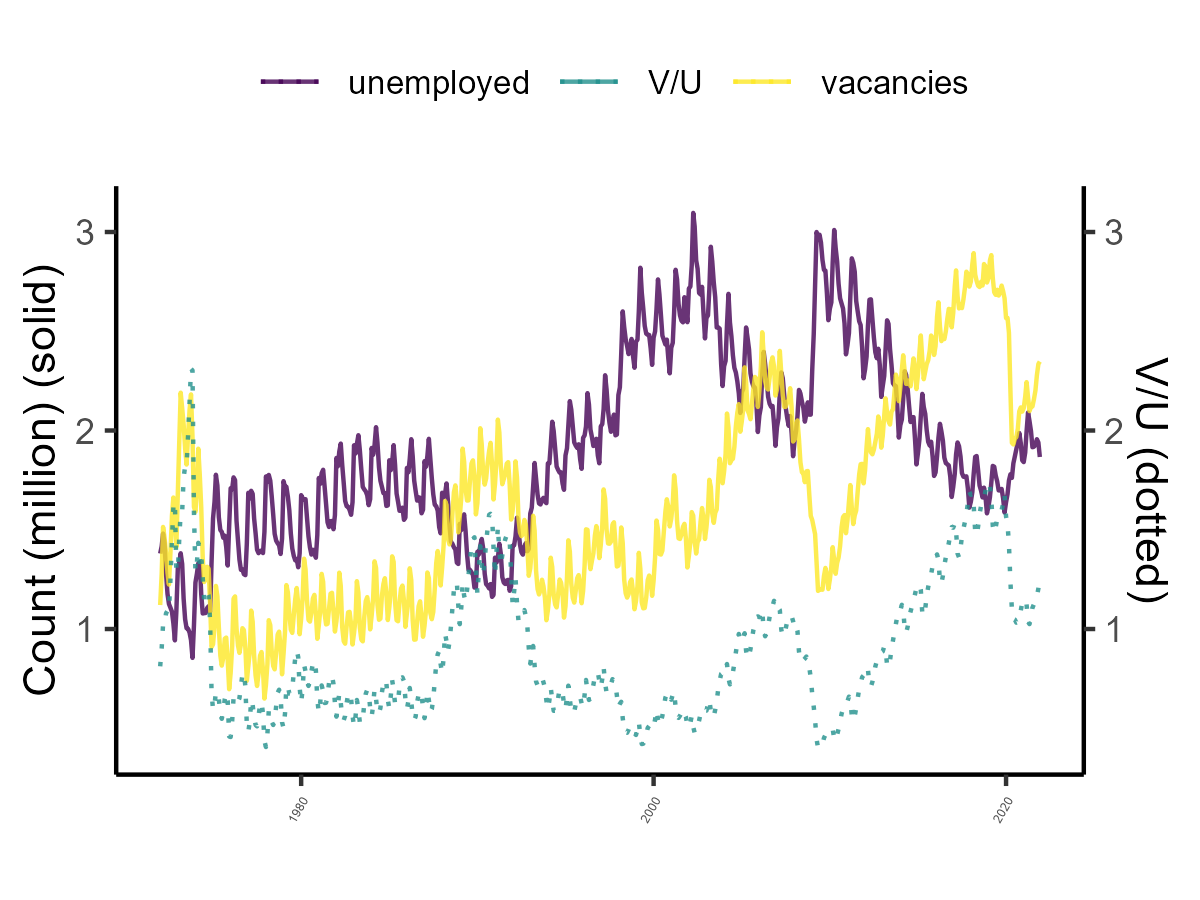
\includegraphics[width = 0.45\textwidth]
  {figuretable/unemployed_vacancy_month_aggregate.png}
  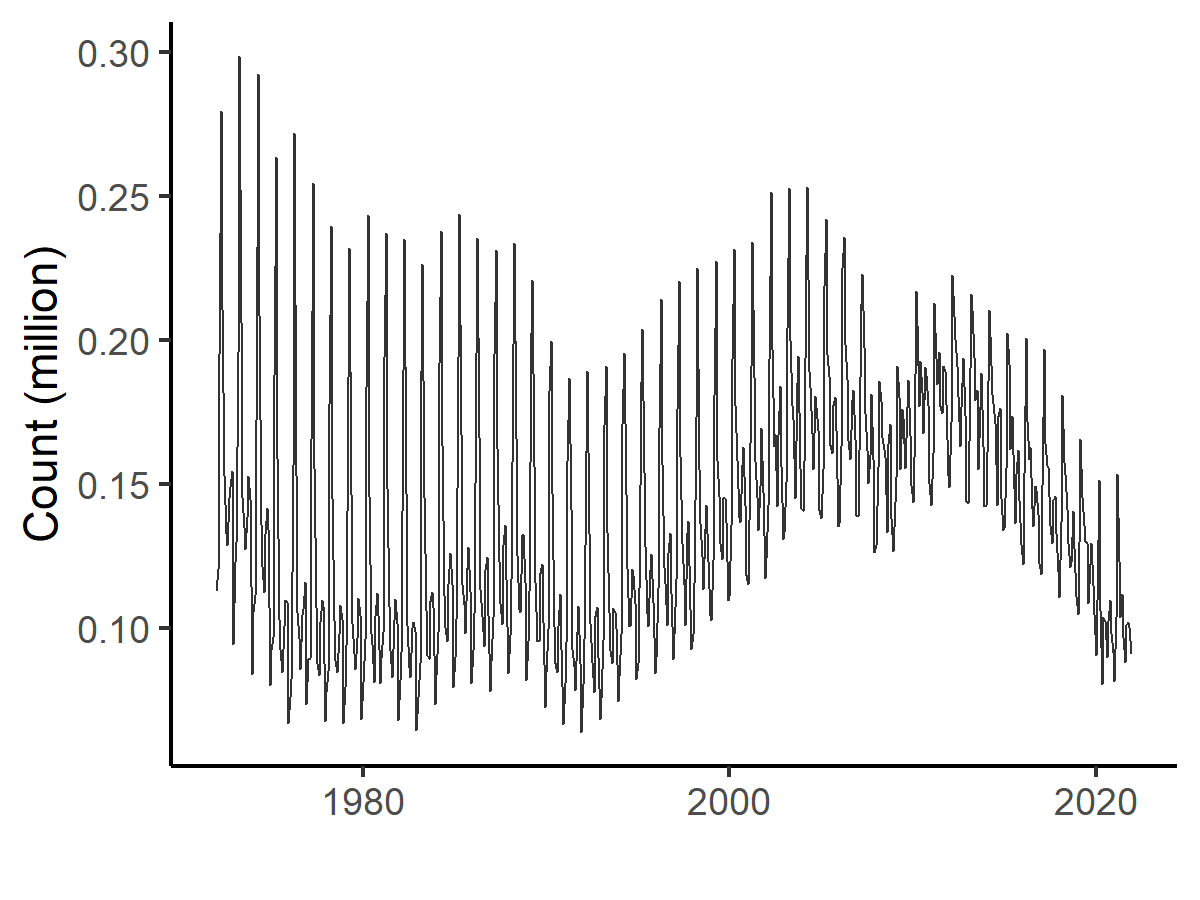
\includegraphics[width = 0.45\textwidth]
  {figuretable/hire_month_aggregate.png}
  \end{center}
  \footnotesize
  %Note: 
\end{figure} 
\begin{itemize}\pause
    \item How does the nonparametric approach work in estimating matching efficiency and mismatch?
    \item What is the trend of \textbf{nonparametric matching efficiency} in Japan in 1973-2024?
    \item What is the trend of \textbf{nonparametric mismatch} in 2013-2023?
\end{itemize}
\end{frame}

\begin{frame}{Main Graphical Takeaway: Estimated Efficiency and Mismatch}
\begin{figure}[!ht]
  \begin{center}
  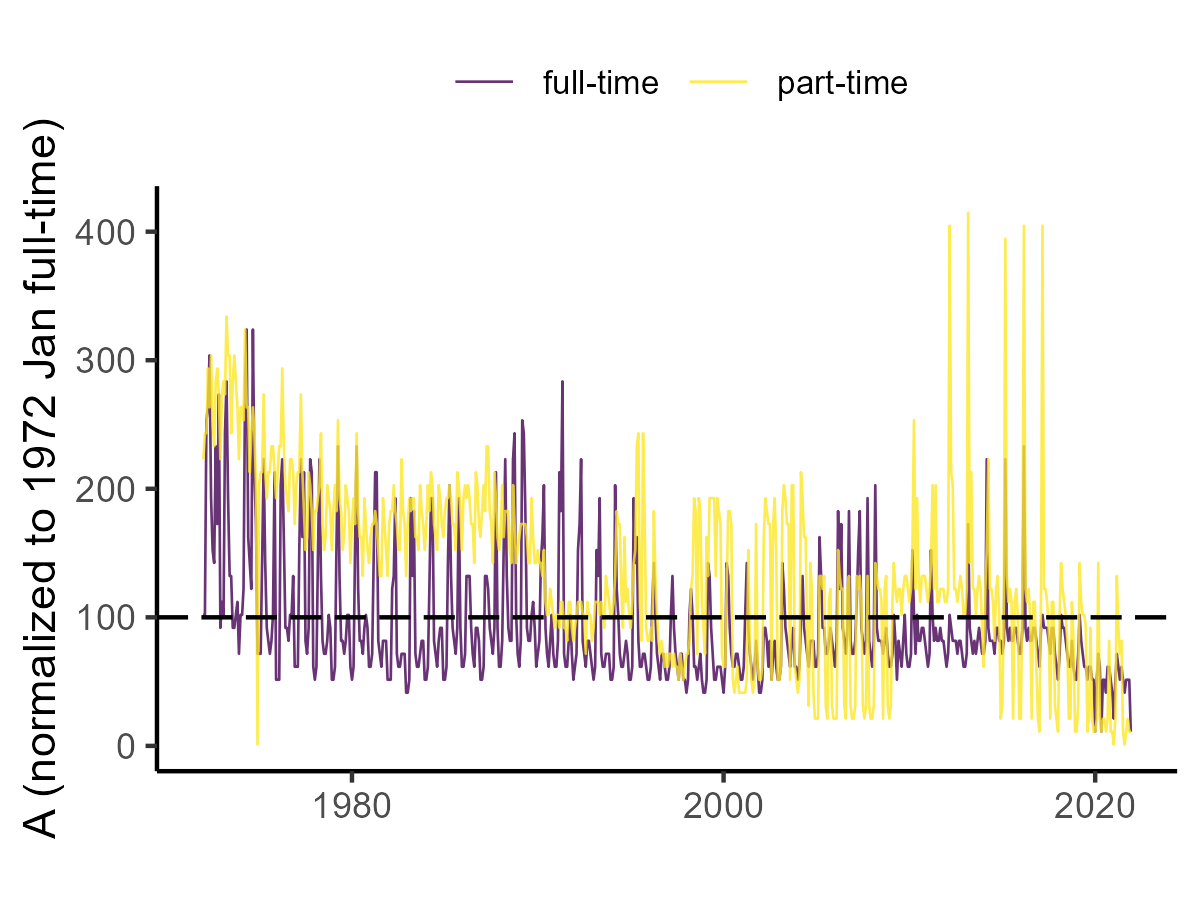
\includegraphics[width = 0.45\textwidth]
  {figuretable/matching_efficiency_month_full_time_part_time.png}
  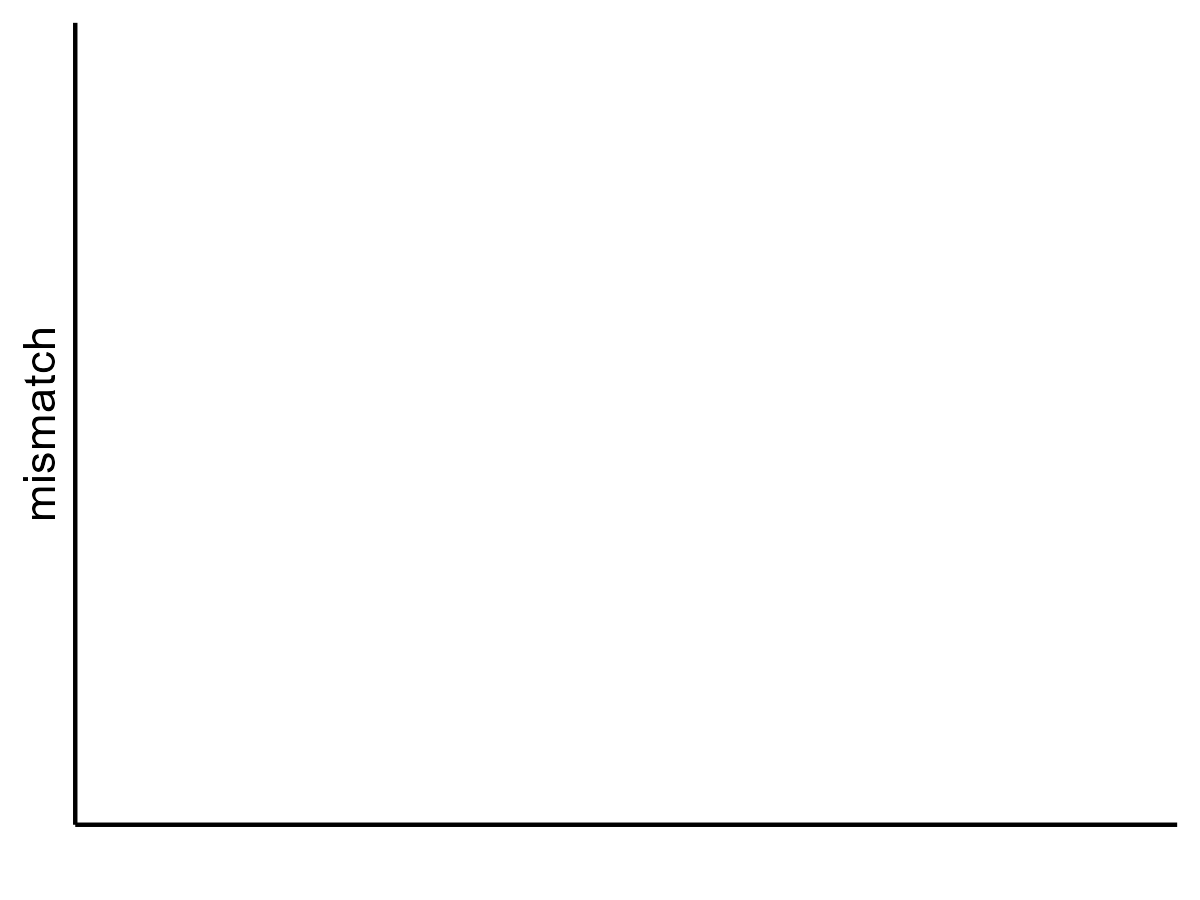
\includegraphics[width = 0.45\textwidth]
  {figuretable/mismatch_part_and_full_time_monthly_job_category.png}
  \end{center}
  \footnotesize
  %Note: 
\end{figure} 
\begin{itemize}
    \item Matching efficiency declines after 2015, driven by both full-time and part-time
    \item Mismatch across job categories increases to 0.3-0.4.
\end{itemize}
\end{frame}

\begin{frame}{Main contributions and findings}
\begin{itemize}
    \item Methodological contribution
    \begin{enumerate}
        \item Examine \textbf{versatility} and \textbf{robustness} of Lange and Papageougeu (2020) and check finite sample performance
        \item Develop \textbf{nonparametric mismatch index,} combining Sahin et al (2014) and MPEC (Su and Judd (2012))
    \end{enumerate}\pause
    \item Empirical findings
    \begin{enumerate}
        \item Japanese labor market via Hello Work in 1966-2024
        \begin{enumerate}
            \item Matching Efficiency \textbf{decreases} driven by both full-time and part-time.
            \item Matching elasticity with respect to unemployed is \textbf{0.5 - 1.1.}
            \item Matching elasticity with respect to vacancies is \textbf{0.03 - 0.5.}
        \end{enumerate}
        \item Japanese prefecture-level and industry-level labor market via Hello Work in 2012-2024
        \begin{enumerate}
            \item Matching Efficiency is\textbf{ higher in rural area (Tohoku) and Agriculture\&Fishery.} 
            \item Elasticities are very heterogeneous.
            \item Mismatch is \textbf{more severe across job categories}.
        \end{enumerate}
    \end{enumerate}
    
\end{itemize}
\end{frame}

\begin{frame}{Related literature}
    \begin{enumerate}
        \item Nonparametric aggregate matching function: Lange\&Papageorgiou (2020, LP)
        \begin{itemize}
            \item Cob Douglass: \textcolor{gray}{Petrongolo and Pissarides (2001), etc}
            \item -> I examine \textbf{versatility} and \textbf{robustness} of LP via simulation
        \end{itemize}
        \item Mismatch: Şahin, Song, Topa, \& Violante (2014, SSTV)
        \begin{itemize}
            \item Cob Douglass: \textcolor{gray}{Patterson et al (2016)}
            \item -> I develop \textbf{a nonparametric mismatch index} combining LP with SSTV.
        \end{itemize}
        \item Japanese Labor market
        \begin{itemize}
            \item Cobb Douglass Matching function: \textcolor{gray}{Kano and Ohta (2005), Kambayashi and Ueno (2006), Sasaki (2008), Higashi (2018,2020,2021)}
            \item Mismatch: \textcolor{gray}{Kawata (2019), Shibata(2020), Higashi and Sasaki (2023)}
            \item -> I apply the above nonparametric method to illustrate \textbf{long-time and short-time trends} of matching efficiency, elasticities, and mismatch.
        \end{itemize}
    \end{enumerate}
\end{frame}

\begin{frame}{Table of contents}
  \setbeamertemplate{section in toc}[sections numbered]
  \tableofcontents%[hideallsubsections]
\end{frame}



\section{Model}

\begin{frame}{Background theory (Rogerson, Shimer, and Wright (2005, JEL))}
    \begin{itemize}
        \item Suppose that at some point in time there are 
        \begin{itemize}
            \item $V$ vacancies posted by firms looking for workers,
            \item $U$ unemployed workers looking for jobs. 
        \end{itemize}
        \item Assume all workers are the same and all firms are homogeneous.
        \item Assume the flow of matches between firms and workers, $H$, is given by a random matching technology $m(\cdot)$.        
        \item The arrival rates for unemployed workers and employers with vacancies are then given by $\frac{H}{U}$ and $\frac{H}{V}$.
        \item Following empirical literature, we treat $m(\cdot)$ as reduced-form exogenous matching function.
    \end{itemize}
\end{frame}


\begin{frame}{Aggregate matching function}
\begin{itemize}
    \item Aggregate matching function $m$ is defined as
    \begin{align*}
        H=m(AU,V)
    \end{align*}
    where $H$ is the number of hires and $m$ satisfies two conditions:
    \begin{enumerate}
        \item \textbf{Constant returns to scale (CRS)}
        \begin{itemize}
            \item Cobb Douglass: $m=AU^{1-\gamma}V^{\gamma}$ with vacancy share $\gamma$
        \end{itemize}
        \item $A\perp V|U$, i.e., \textbf{independence between $A$ and $V$ conditional on $U$}
    \end{enumerate}
    
        \item Our goal is to \textbf{recover unobserved $A$ from observed $(H,U,V)$.}
\end{itemize}
    
\end{frame}

\begin{frame}{A social planner problem}
    \begin{itemize}
    \item Suppose there are $G$ isolated markets in time $t$. 
    \item The number of hires $H_{g t}$ in market $g$ in time $t$ is determined by a matching function $$m\left(A_{g t} U_{g t}, V_{g t}\right)$$
    \item A social planner maximizes the total hires in the economy \textbf{by distributing a given number of unemployed workers to each labor market.}
    \item Assume homogenous productivity and job separation rate across labor markets.
\end{itemize}
\end{frame}

\begin{frame}{Optimal unemployed (Sahin et al (2014))}
    \begin{itemize}
    \item Define mismatch as \textbf{the deviation of the hires in the data from the efficient allocation chosen by the social planner}. 
    
    \item The optimal allocation of unemployed workers $U^*$ satisfies:
    $$
    \frac{\partial m}{\partial U}\left(A_{1 t} U_{1 t}^*, V_{1 t}\right)=\cdots=\frac{\partial m}{\partial U}\left(A_{G t} U_{G t}^*, V_{G t}\right)
    $$
    where * denotes the planner's allocation.
    \begin{itemize}
        \item Keeping total unemployed workers $U_t=\sum_{g=1}^G U_{g t}$, the planner allocates more unemployed workers to more effective labor markets%, that is, with more vacancies and higher matching efficiency until their marginal contribution to the hires is equalized across markets. 
    \end{itemize}
    \item The main difference from Sahin et al. (2014) is that equilibrium condition \textbf{does not have an analytical formula} like Cobb Douglas specification:
    \begin{align*}
        A_{m}A_{t}\left(\frac{V_{m t}}{U_{m t}^{\star}}\right)^\gamma (1-\gamma)=A_{m'}A_{t}\left(\frac{V_{m' t}}{U_{m' t}^{\star}}\right)^\gamma (1-\gamma)
    \end{align*}
\end{itemize}
\end{frame}


\begin{frame}{Mismatch}
    \begin{itemize}
    \item Using optimal allocation of unemployed workers $U_{g t}^*$, the aggregate actual and optimal number of new hires can be expressed as
$$
\begin{aligned}
H_t & =\sum_{g=1}^G m\left(A_{g t} U_{g t}, V_{g t}\right) \\
H_t^* & =\sum_{g=1}^G m\left(A_{g t} U_{g t}^*, V_{g t}\right)
\end{aligned}
$$
\item I define mismatch index as the fraction of hires lost because of misallocation:
$$
\mathcal{M}_t=1-\frac{H_t}{H_t^*}
$$

\item This index accounts for \textbf{the heterogeneity of matching efficiencies across labor markets.}
\end{itemize}
\end{frame}

\begin{frame}{Why nonparametric is better than Cobb Douglass with fixed effects?}
\begin{itemize}
    \item Suppose that we observe $M$ markets in $T$ years.
    \begin{enumerate}
        \item Cobb Douglass specification estimates $T+M+1$ parameters.
        \begin{itemize}
        \item $T$ year fixed effects.
        \item $M$ market fixed effects.
        \item constant vacancy share parameter $\gamma$.
        \item Nonparametric approach estimates $T\times M$ efficiencies corresponding time-varying elasticities.
        \end{itemize}
        \item Cobb Douglass mismatch cancels out time variations of $A_{t}$ and elasticity:
        \begin{align*}
        A_{m}\textcolor{red}{A_{t}}\left(\frac{V_{m t}}{U_{m t}^{\star}}\right)^\gamma \textcolor{red}{(1-\gamma)}=A_{m'}\textcolor{red}{A_{t}}\left(\frac{V_{m' t}}{U_{m' t}^{\star}}\right)^\gamma\textcolor{red}{ (1-\gamma)}
    \end{align*}
    \end{enumerate}
    
    \item Trade-off: \textbf{``Much more" flexibility vs sample size}
    \begin{itemize}
        \item We want to check finite sample performance.
    \end{itemize}
\end{itemize}
    
\end{frame}



\section{Identification, Estimation, and Computation}

\begin{frame}{Intuition}
    \begin{itemize}
    \item Three markets example.
    \end{itemize}
    \begin{enumerate}
        \item If $(U,V,A)=(100,100,A_0)$ at $t=0$, $m(AU,V)=15$. (normalization point)\pause
        \item If $(U,V,A)=(100,100,?)$ at $t=1$, $m(AU,V)=10$.\pause
        \begin{itemize}
            \item $?$ must be smaller than $A_0$\pause
        \end{itemize}
        \item If $(U,V,A)=(90,100,?)$ at $t=2$, $m(AU,V)=15$.\pause
        \begin{itemize}
            \item $?$ must be larger than $A_0$\pause
        \end{itemize}
    \end{enumerate}
    \begin{itemize}
        \item Pooling all $T$ markets, we check this at each $t$ repeatedly.
    \end{itemize}
\end{frame}

\begin{frame}{Nonparametric identification}
    \begin{itemize}
    \item Denote by $F(A, U)$ the joint distribution of $A$ and $U$. 
    \item Denote by $G(H, U, V)$ the joint distribution of $(H,U,V)$.
    \item Applying Matzkin (2003), LP shows that \textbf{$G(H, U, V)$ identifies $F(A, U)$ and $m(A U, V)$ up to a normalization of $A$ at one point of the support of $(H, U, V)$.}\pause
    \item Key transformation:
    \begin{align*}
        F(\underbrace{A}_{\text{unobserved}} \mid \underbrace{U}_{\text{observed}})&=\quad F(A \mid U, V) \quad \text { by independence of } A \perp V \mid U \\
        & =\operatorname{Pr}(h \leq m(A U, V) \mid U, V) \text { by monotonicity } \\ 
        & =\operatorname{Pr}(h \leq H \mid U, V) \\ 
        & =\quad G_{H \mid U, V}\underbrace{(H \mid U, V)}_{\text{observed}}
    \end{align*}
    \end{itemize}
\end{frame}

\begin{frame}{Nonparametric estimation \textcolor{red}{[For reference]}}
    \begin{itemize}
    \item First estimate a constructive estimator $\hat{F}(A_t|U_t)=G\left(H_t \mid U_t, V_t\right)$ 
    \begin{itemize}
        \item using bivariate kernels.
    \end{itemize}
    \item Second, recover $\hat{A}_t=\hat{F}^{-1}\left(G\left(H_t \mid U_t, V_t\right) \mid U_t\right)$.
    \item Third, recover $m\left(\hat{A}_t U_t, V_t\right)=G^{-1}\left(\hat{F}\left(\hat{A}_t \mid U_t\right) \mid U_t, V_t\right)$.
    \begin{itemize}
        \item To approximate $\frac{d m}{d AU}$ and $\frac{d m}{d V}$, I run LASSO regression of $H_{t}$ on second order polynomial of $\hat{A_{t}}U_{t}$ and $V_{t}$.
    \end{itemize}
    
    
    \end{itemize}
\end{frame}

\begin{frame}{Computation mismatch}
    \begin{itemize}
    \item The planner allocates unemployed workers satisfying the equilibrium conditions:
    $$
    \frac{\partial m}{\partial U}\left(A_{1 t} U_{1 t}^*, V_{1 t}\right)=\cdots=\frac{\partial m}{\partial U}\left(A_{G t} U_{G t}^*, V_{G t}\right)
    $$
    keeping total unemployed workers $U_t=\sum_{g=1}^G U_{g t}$
    \item This can be represented as a \textbf{nonlinear system of equations with linear equilibrium constraints}.
    \item Can be solved by \textbf{MPEC} (Mathematical Programming with Equilibrium Constraint) proposed by Su and Judd (2012) and Dube, Fox, and Su (2012).
    \begin{itemize}
        \item Allow incorporating richer elements.
    \end{itemize}
    \item After getting $U^*$, we calculate mismatch $\mathcal{M}_t$.
    \end{itemize}
\end{frame}



\section{Monte Carlo simulation results}

\begin{frame}{Motivation for finite sample performance}
\begin{itemize}
    %\item We want to check \textbf{robustness} to specification, stationarity, and endogeneity.
    \item We want to check \textbf{robustness} to specification and endogeneity.
    \begin{enumerate}
        \item Restricting CRS class including Cobb Douglas.
        %\item Experiment stationary ARIMA(1,0,0) and nonstationary ARIMA(0,1,0)
        \item Check robustness to violation of independence of $A$ and $V$ conditional on $U$.
    \end{enumerate}
    \item We want to confirm how large enough the sample size is.
    \item We want to quantify the bias of the standard Cobb Douglass specification \textcolor{blue}{[Skipped]}
\end{itemize}
    
\end{frame}

\begin{frame}{Setup: DGP}
\begin{itemize}
    \item Sample size $T=50,100$
    \item $(U,V,A)$ is generated in AR(1) with auto correlation $0.2$.
    \item CRS class specification of $m$
    \begin{itemize}
        \item Cobb Douglas: $(AU)^{\gamma}V^{1-\gamma}$ with $\gamma=0.7$
        \item Perfect substitute: $\gamma AU+\gamma V$ \textcolor{blue}{[Skipped because of similar results]}
    \end{itemize}
    % \item Stationarity of $A$: ($U$ and $V$ are stationary now)
    % \begin{itemize}
    %     \item ARIMA(1,0,0)
    %     \item ARIMA(0,1,0)
    % \end{itemize}
    \item Endogeneity of $(A,U,V)$
    \begin{itemize}
        \item Use choresky decomposition of $A$ and $V$ where $q=0$ (independence), $0.1, 0.2$.
    \end{itemize}
    \item Other tuning parameter: kernel choice and bandwidth.
    \item Level and scale normalization is implemented to avoid negative values.
    \item \textcolor{blue}{Detailed Monte Carlo simulation is under construction}
    \item Pick one simulation path for illustration.
\end{itemize}
    
\end{frame}

\begin{frame}{Illustrative fitting plot: Sample size}
\begin{figure}[!ht]
  \begin{center}

  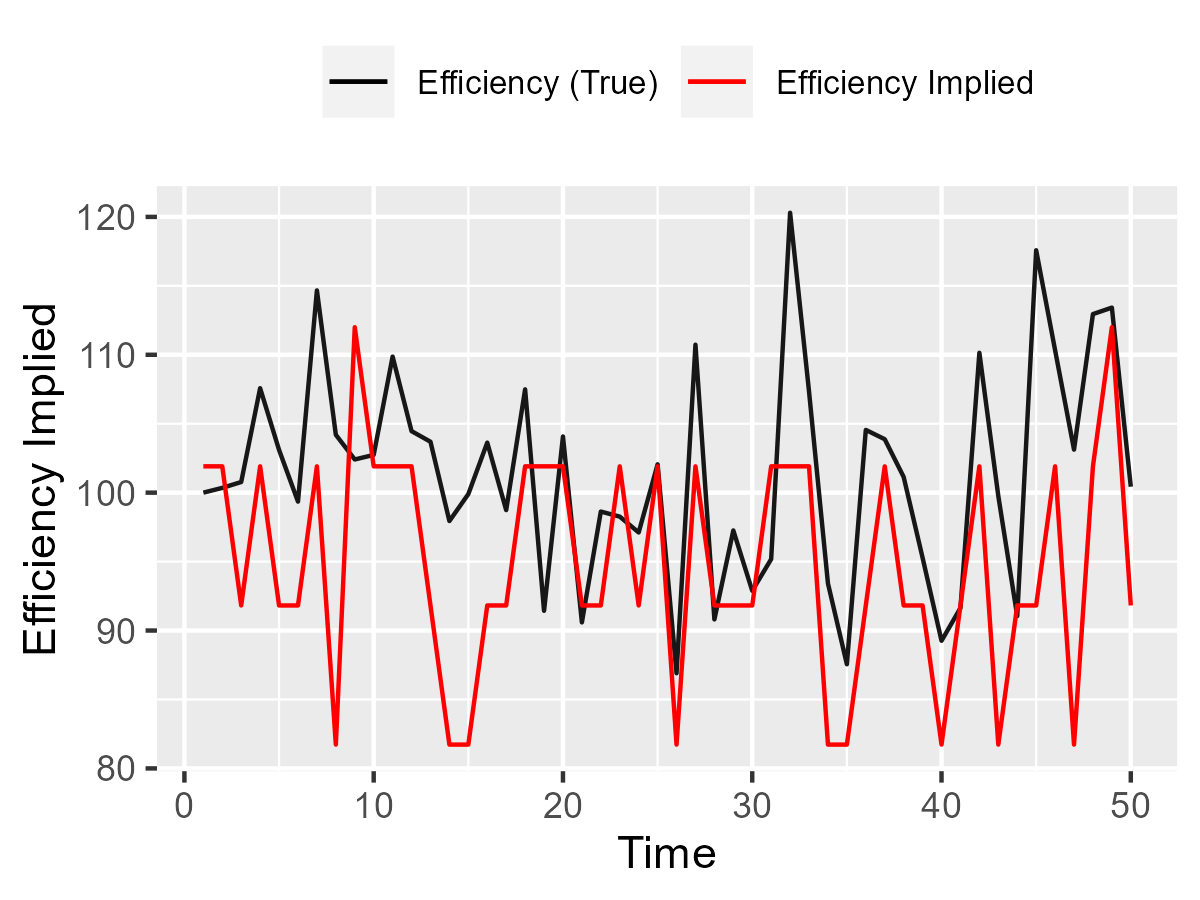
\includegraphics[width = 0.45\textwidth]
  {figuretable/illustrative_plot_implied_efficiency_num_time_50_cobb_douglas_0.3_AR1_I0_va_dependency_0.png}
  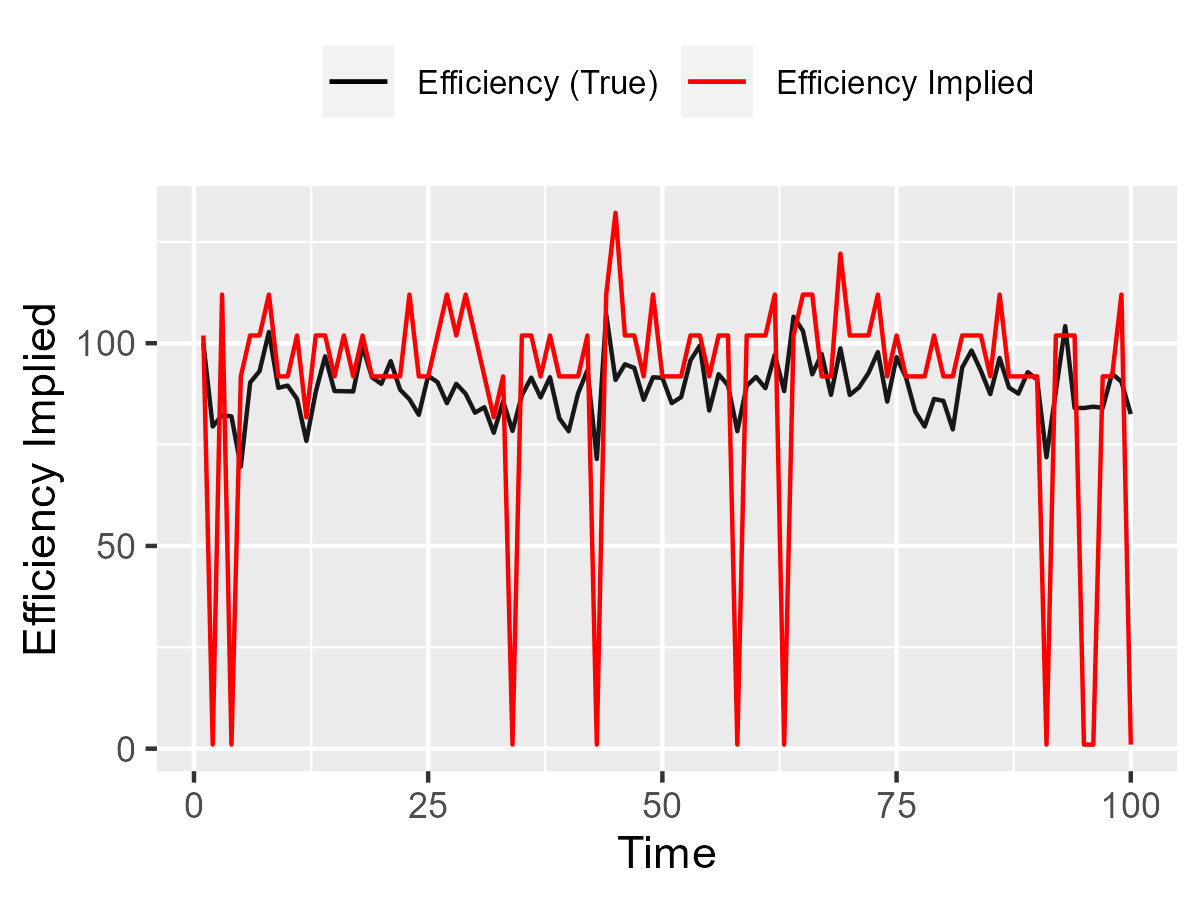
\includegraphics[width = 0.45\textwidth]
  {figuretable/illustrative_plot_implied_efficiency_num_time_100_cobb_douglas_0.3_AR1_I0_va_dependency_0.png}
  \end{center}
  \footnotesize
  %Note: 
\end{figure}
\begin{itemize}
     \item $T=100$ seems enough.
     \item Bias and RMSE decreases as $T$ increases. 
     \item Some outlier estimates are observed but easily detected.
\end{itemize}
\end{frame}

% \begin{frame}{Illustrative fitting plot: Without stationary of $A$}
% \begin{figure}[!ht]
%   \begin{center}

%   \includegraphics[width = 0.45\textwidth]
%   {figuretable/illustrative_plot_implied_efficiency_num_time_50_cobb_douglas_0.3_AR0_I1_va_dependency_0.png}
%   \includegraphics[width = 0.45\textwidth]
%   {figuretable/illustrative_plot_implied_efficiency_num_time_100_cobb_douglas_0.3_AR0_I1_va_dependency_0.png}
%   \end{center}
%   \footnotesize
%   %Note: 
% \end{figure} 
% \begin{itemize}
%     \item Long nonstationarity gives fluctuate estimates.
%     \item So, bias and RMSE increases as $T$ increases. 
%     %\item However, the estimate captures the smooth trend reasonably.
% \end{itemize}
% \end{frame}

\begin{frame}{Illustrative fitting plot: Without endogeneity, 0.1 (left) and 0.2 (right)}
\begin{figure}[!ht]
  \begin{center}
  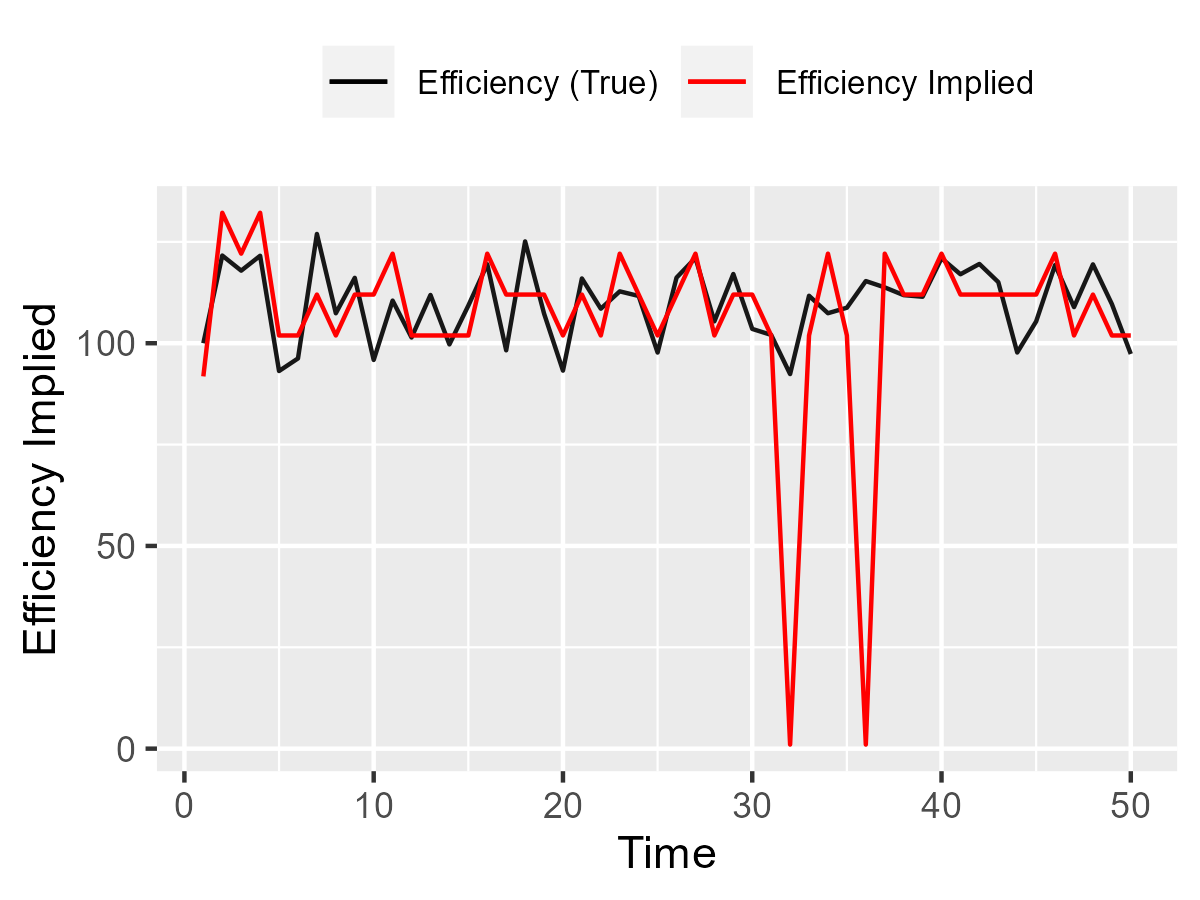
\includegraphics[width = 0.30\textwidth]
  {figuretable/illustrative_plot_implied_efficiency_num_time_50_cobb_douglas_0.3_AR1_I0_va_dependency_0.1.png}
  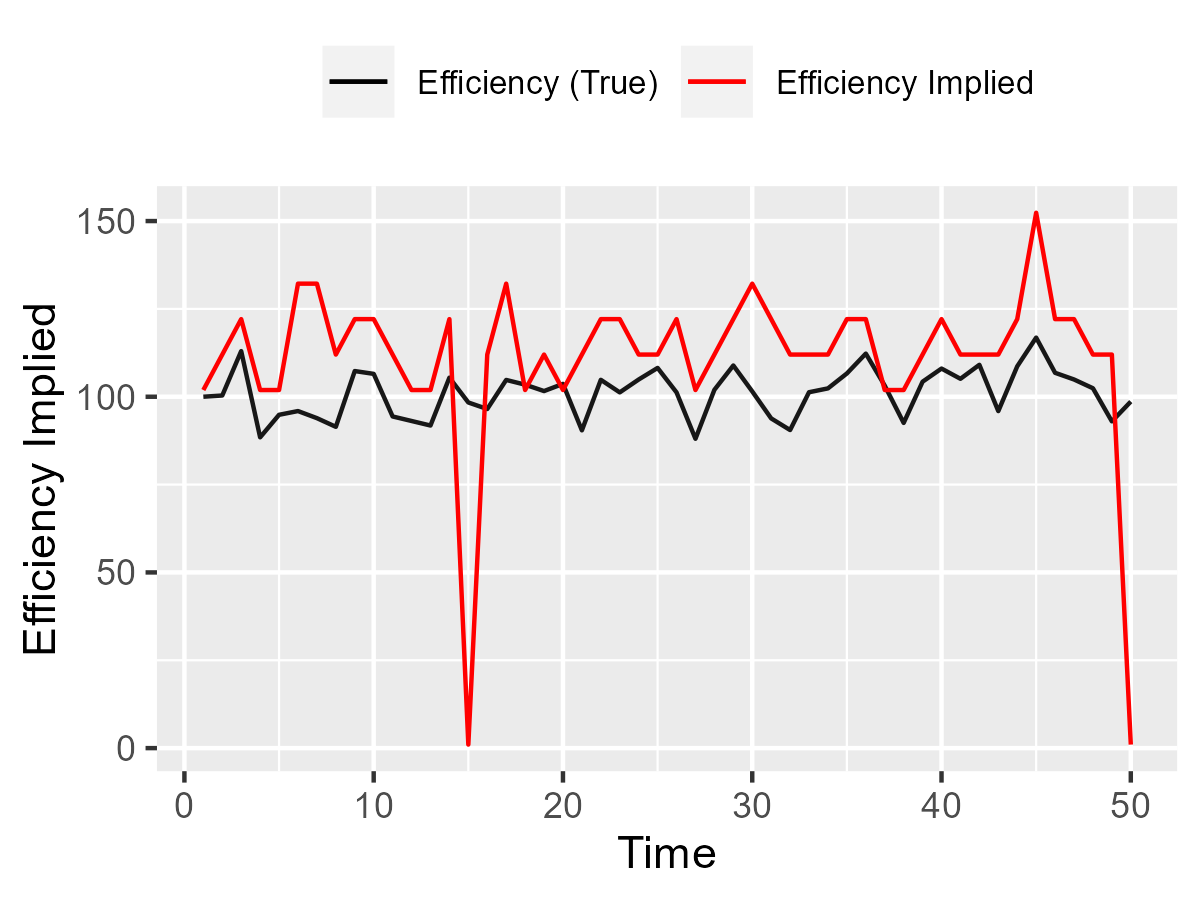
\includegraphics[width = 0.30\textwidth]
  {figuretable/illustrative_plot_implied_efficiency_num_time_50_cobb_douglas_0.3_AR1_I0_va_dependency_0.2.png}\\

  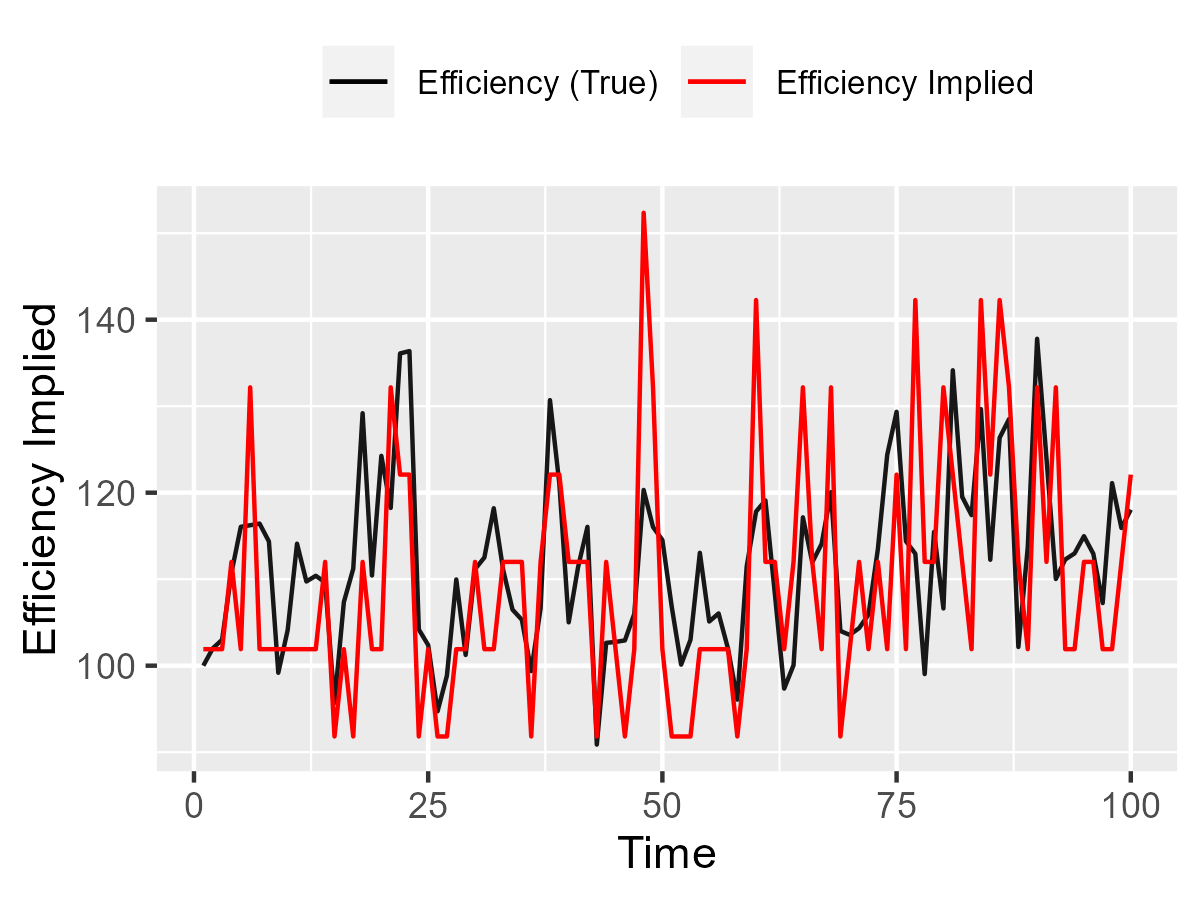
\includegraphics[width = 0.30\textwidth]
  {figuretable/illustrative_plot_implied_efficiency_num_time_100_cobb_douglas_0.3_AR1_I0_va_dependency_0.1.png}
  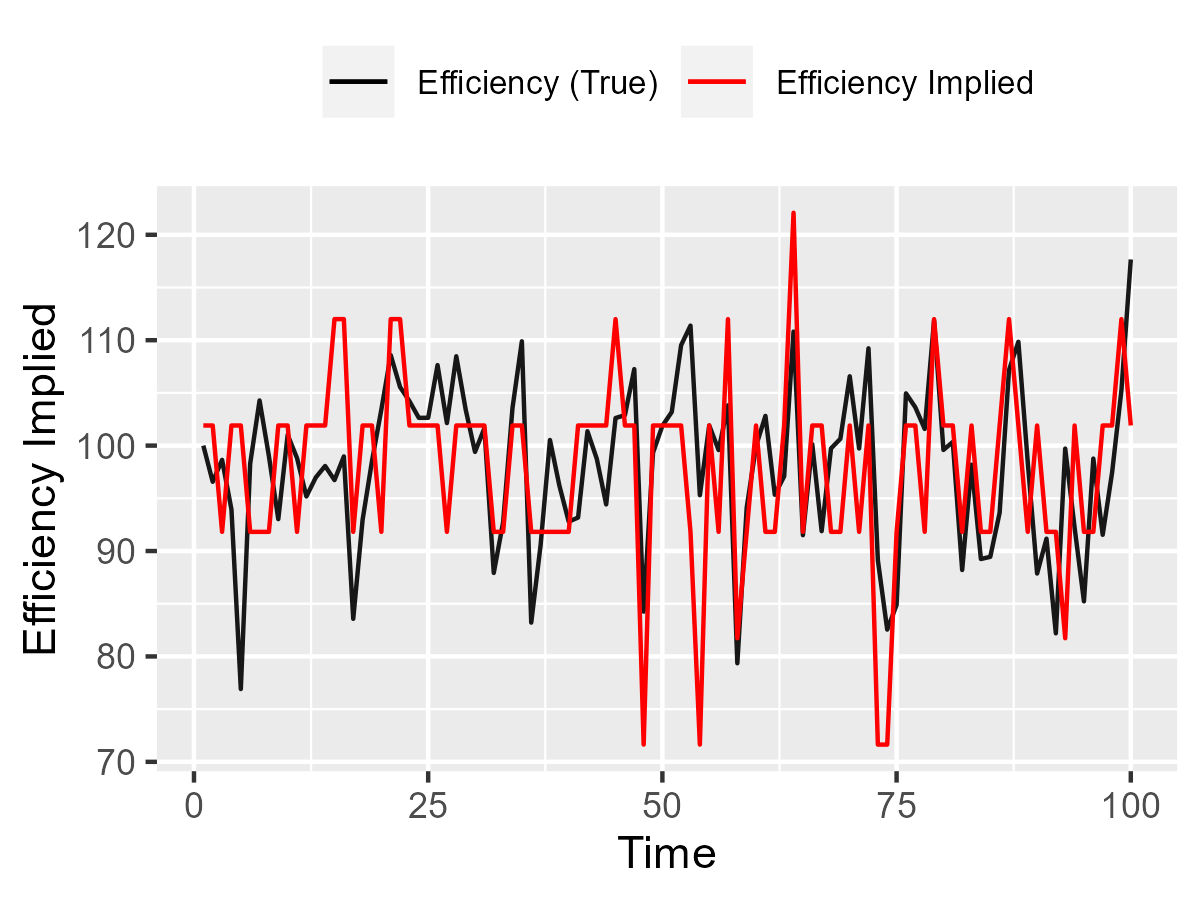
\includegraphics[width = 0.30\textwidth]
  {figuretable/illustrative_plot_implied_efficiency_num_time_100_cobb_douglas_0.3_AR1_I0_va_dependency_0.2.png}
  \end{center}
  \footnotesize
  %Note: 
\end{figure} 
\begin{itemize}
    \item Small endogeneity seems not so harmful (bias<$1\%$) in $T=100$.
\end{itemize}
\end{frame}

\begin{frame}{Summary of Monte Carlo simulation results}
\begin{itemize}
    \item Sample size $t=100$ seems enough.
    \item Robust to specification of $m$.
    \item Seemingly robust to endogeneity of $A$ and $V$.
    %\item But, \textbf{sensitive} to stationary assumption on efficiency $A$
\end{itemize}
    
\end{frame}






\section{Empirical Results: 1966-2023}

\begin{frame}{Data}
  \begin{itemize}
      \item Hello Work data via Public Employment Office in Japan
      \begin{itemize}
          \item About 80\% of unemployed and 20\% of hires are covered in Japan.
          \item Observe part-time, full-time, its aggregate.
      \end{itemize}
      \item Observed variables in each market
      \begin{itemize}
          \item Unemployed
          \item Vacancy
          \item Hire
      \end{itemize}
      \item Target period
      \begin{itemize}
          \item Long time trend study: Country-month-level in 1973-2024.
          \item Short time trend study: Industry(large job category)-month-level in 2012-2024 and prefecture-month-level in 2013-2024.
      \end{itemize}
      
  \end{itemize}
\end{frame}

\begin{frame}{Overview of the first empirical exercise}
    \begin{itemize}
        \item Data: Country-year-level data in 1973-2023.
        \item Estimate matching efficiency for each dataset
        \begin{enumerate}
            \item All (=Full-time + Part-time)
            \item Decompose Full-time and Part-time
        \end{enumerate}
    \end{itemize}
\end{frame}

\begin{frame}{Residual plot to check endogeneity \textcolor{red}{[For reference]}}
    \begin{figure}[!ht]
  \begin{center}
  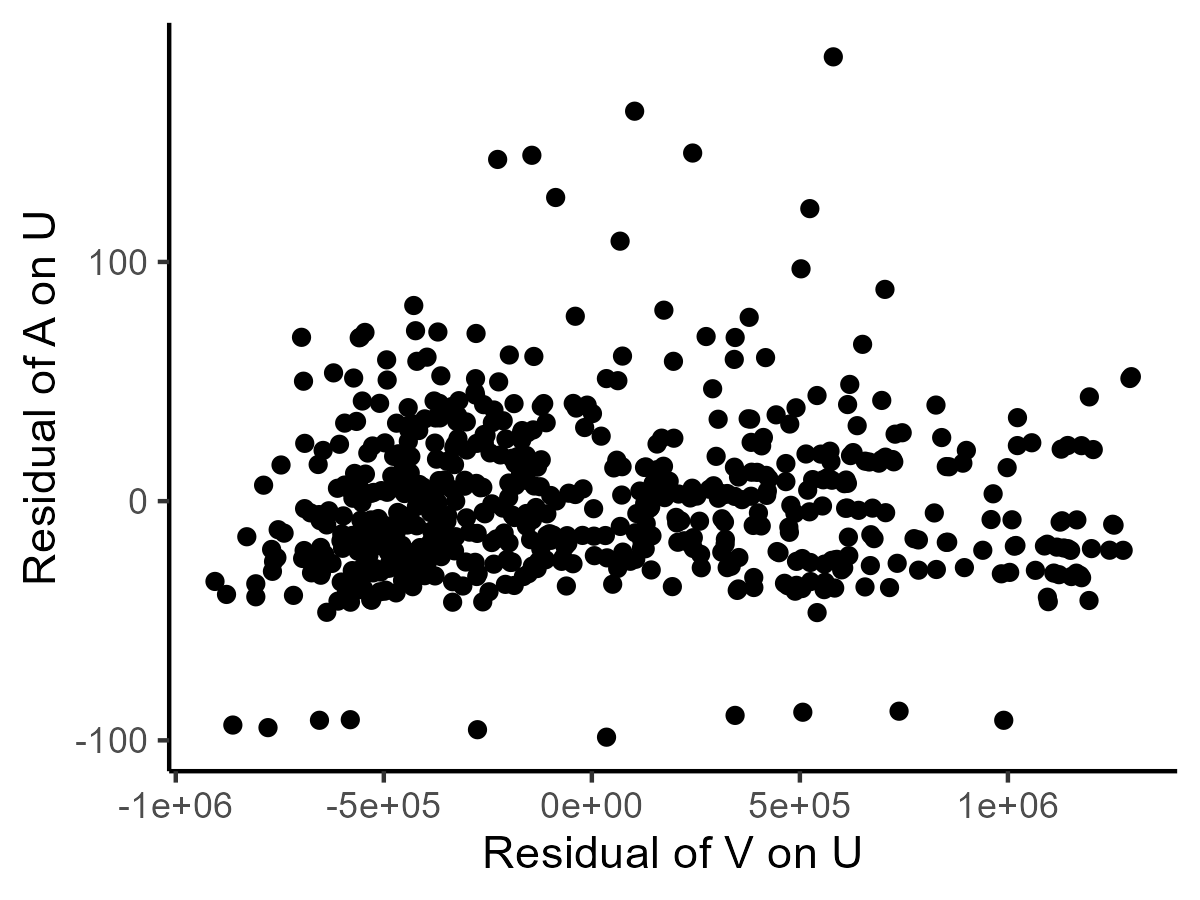
\includegraphics[width = 0.50\textwidth]
  {figuretable/residual_plot_month_aggregate.png}
  \end{center}
  \footnotesize
  %Note: 
\end{figure} 
\begin{itemize}
    \item Correlation of residuals (=0.04) seems not significant.
\end{itemize}
\end{frame}



\begin{frame}{Fact: $U,V,H$ and Tightness $V/U$}
    \begin{figure}[!ht]
  \begin{center}
  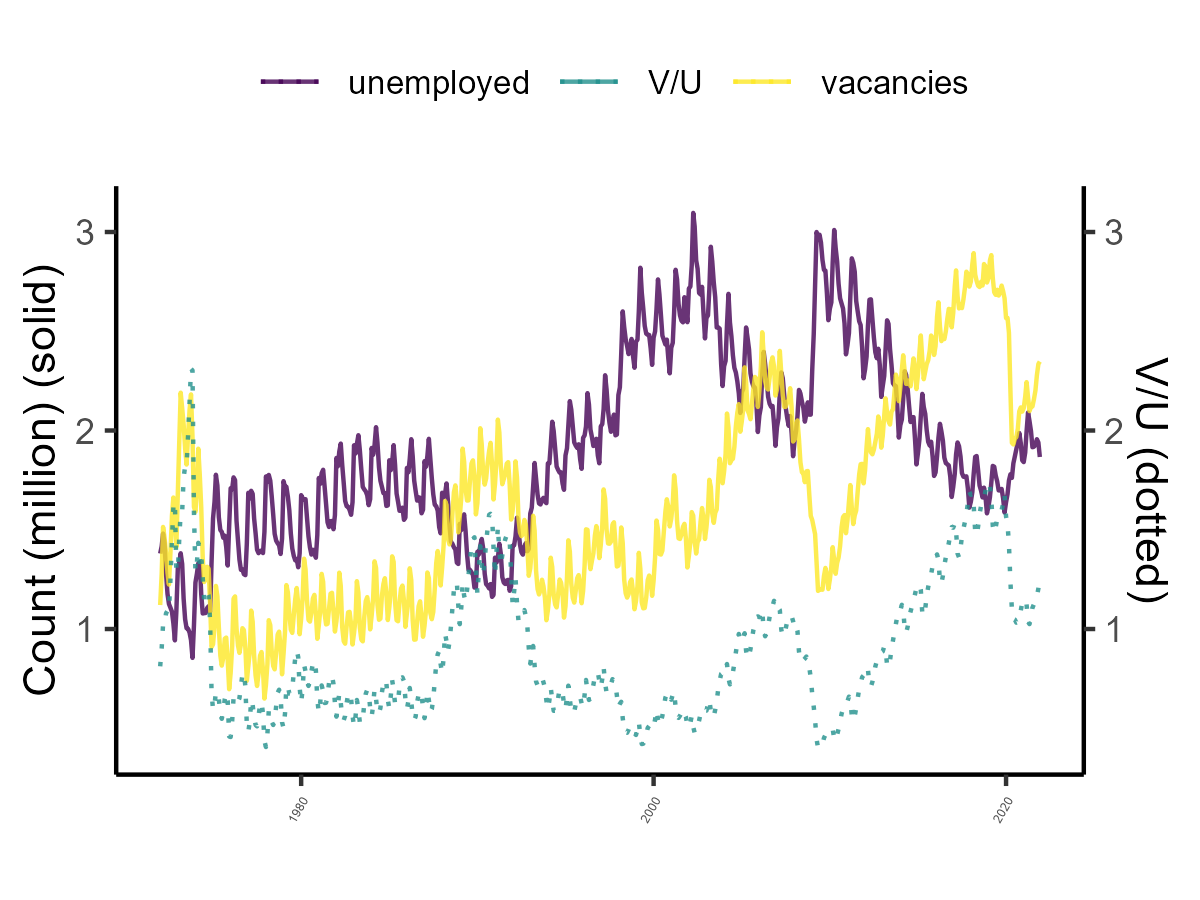
\includegraphics[width = 0.3\textwidth]
  {figuretable/unemployed_vacancy_month_aggregate.png}
  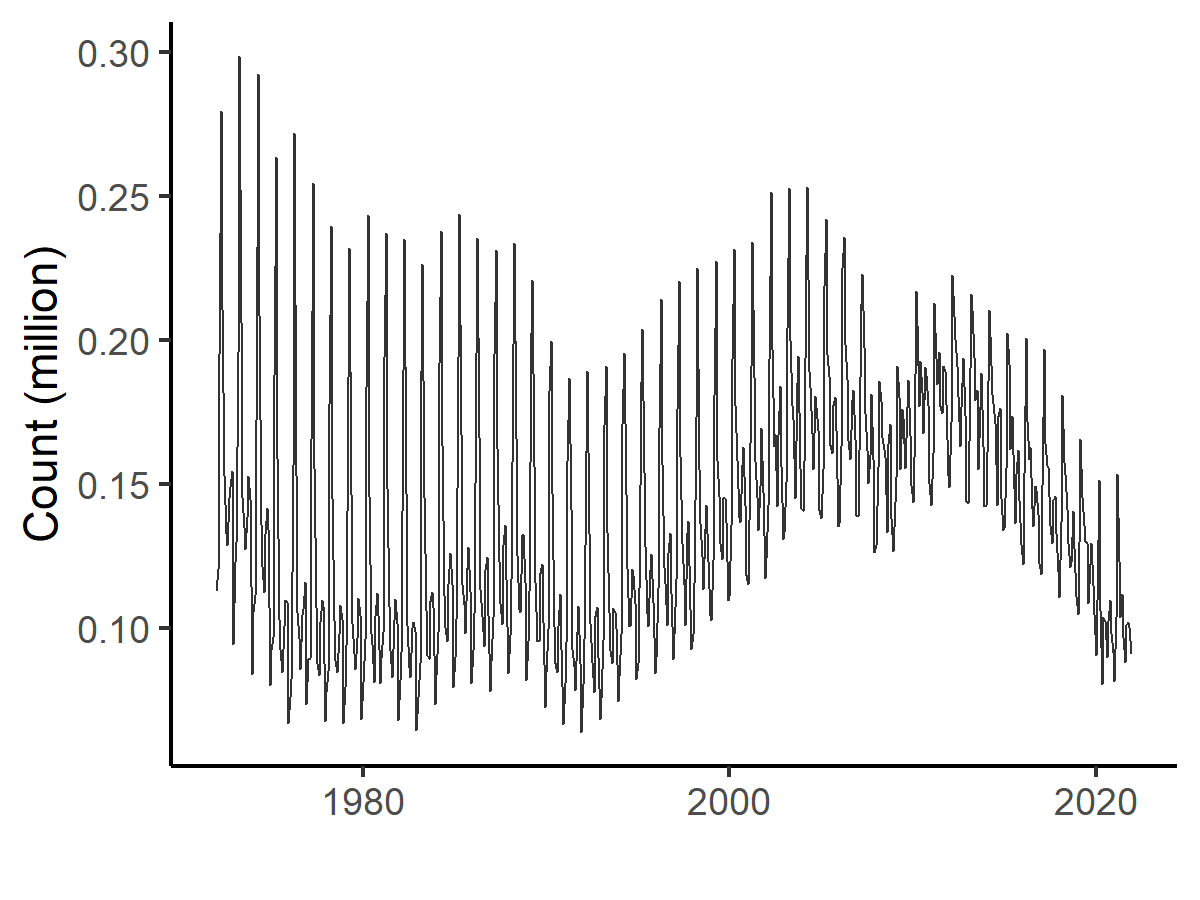
\includegraphics[width = 0.3\textwidth]
  {figuretable/hire_month_aggregate.png}
  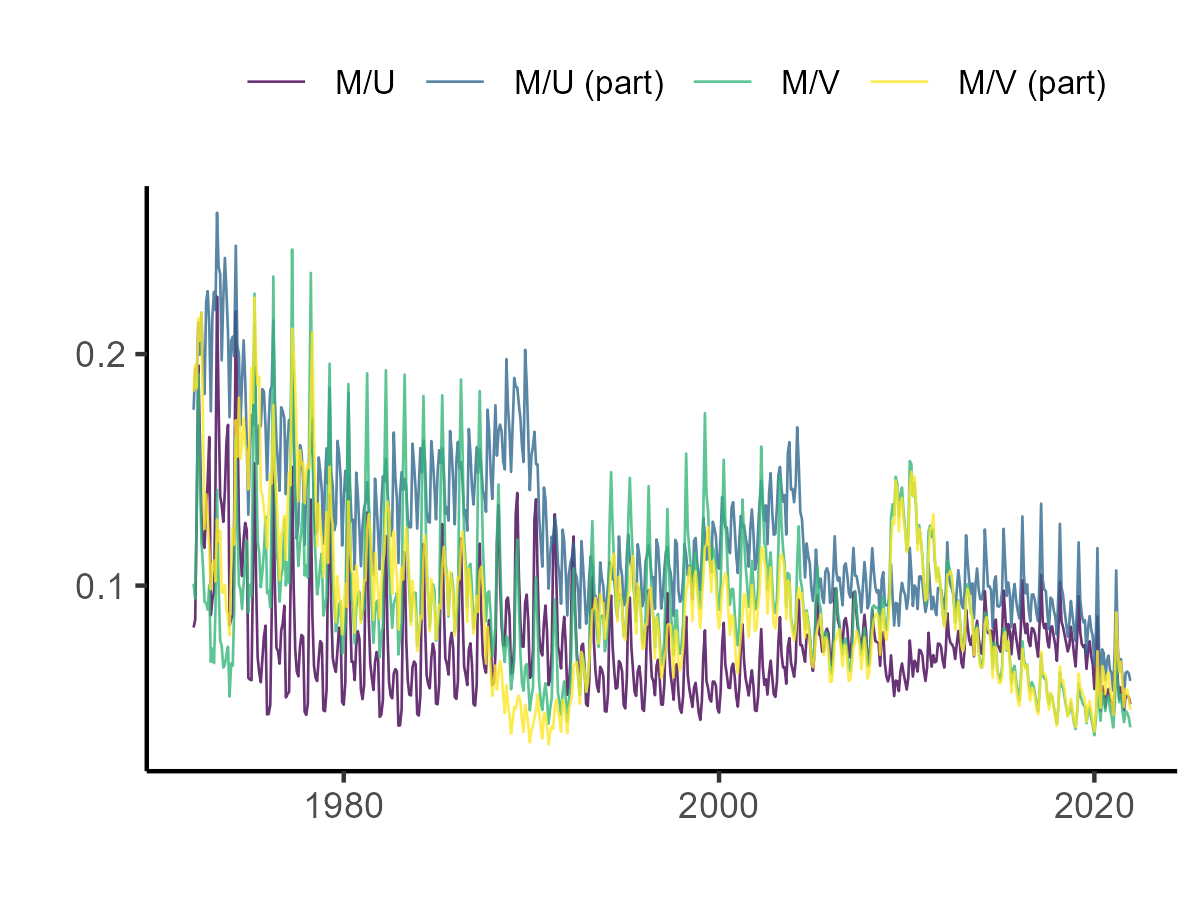
\includegraphics[width = 0.3\textwidth]
  {figuretable/job_finding_rate_worker_finding_rate_month_aggregate.png}
  \end{center}
  \footnotesize
  %Note: 
\end{figure} 
\begin{itemize}
    \item $U,V,H$ show cyclicality.
    \item Job-finding rate and Worker-finding rate decrease gradually.
\end{itemize}
\end{frame}

\begin{frame}{Matching Efficiency and Elasticities}
    \begin{figure}[!ht]
  \begin{center}
  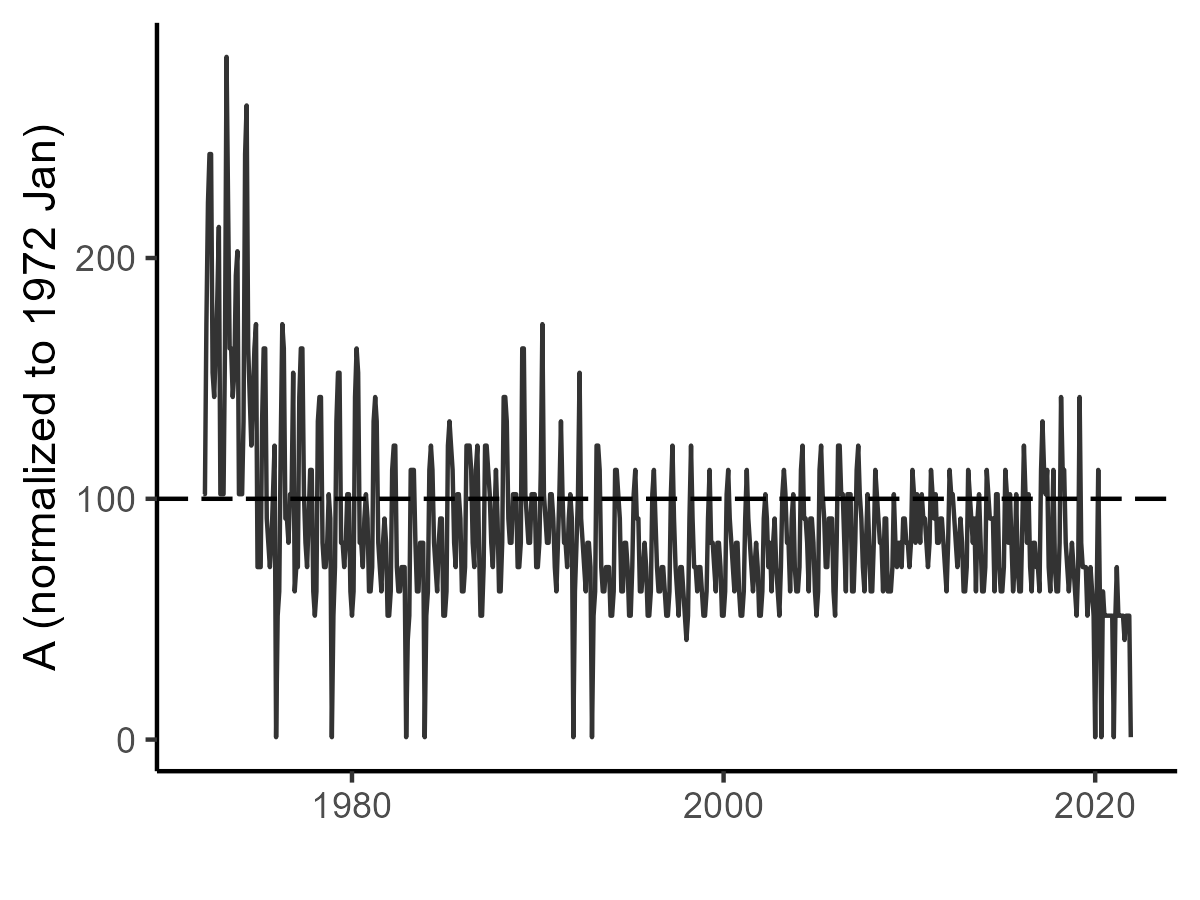
\includegraphics[width = 0.45\textwidth]
  {figuretable/matching_efficiency_month_aggregate.png}
  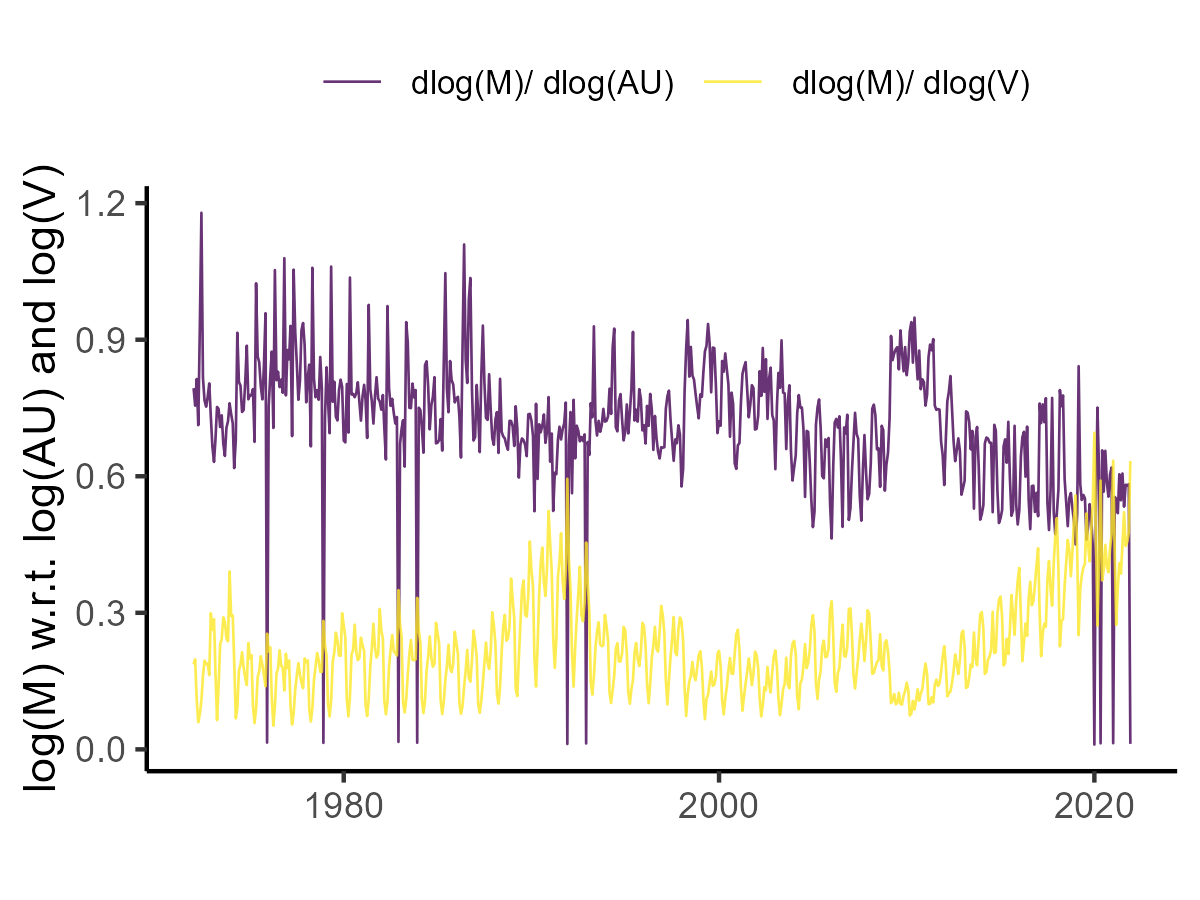
\includegraphics[width = 0.45\textwidth]
  {figuretable/elasticity_month_aggregate.png}
  \end{center}
  \footnotesize
  %Note: 
\end{figure} 
\begin{itemize}
    \item Matching efficiency declines after 2015.
    \item Matching elasticity with respect to unemployed is 0.5 - 1.1.
    \item Matching elasticity with respect to vacancies is 0.03 - 0.5. (0.15-0.3 in U.S.)
\end{itemize}
\end{frame}

\begin{frame}{Correlation of Efficiency and Tightness}
    \begin{figure}[!ht]
  \begin{center}
  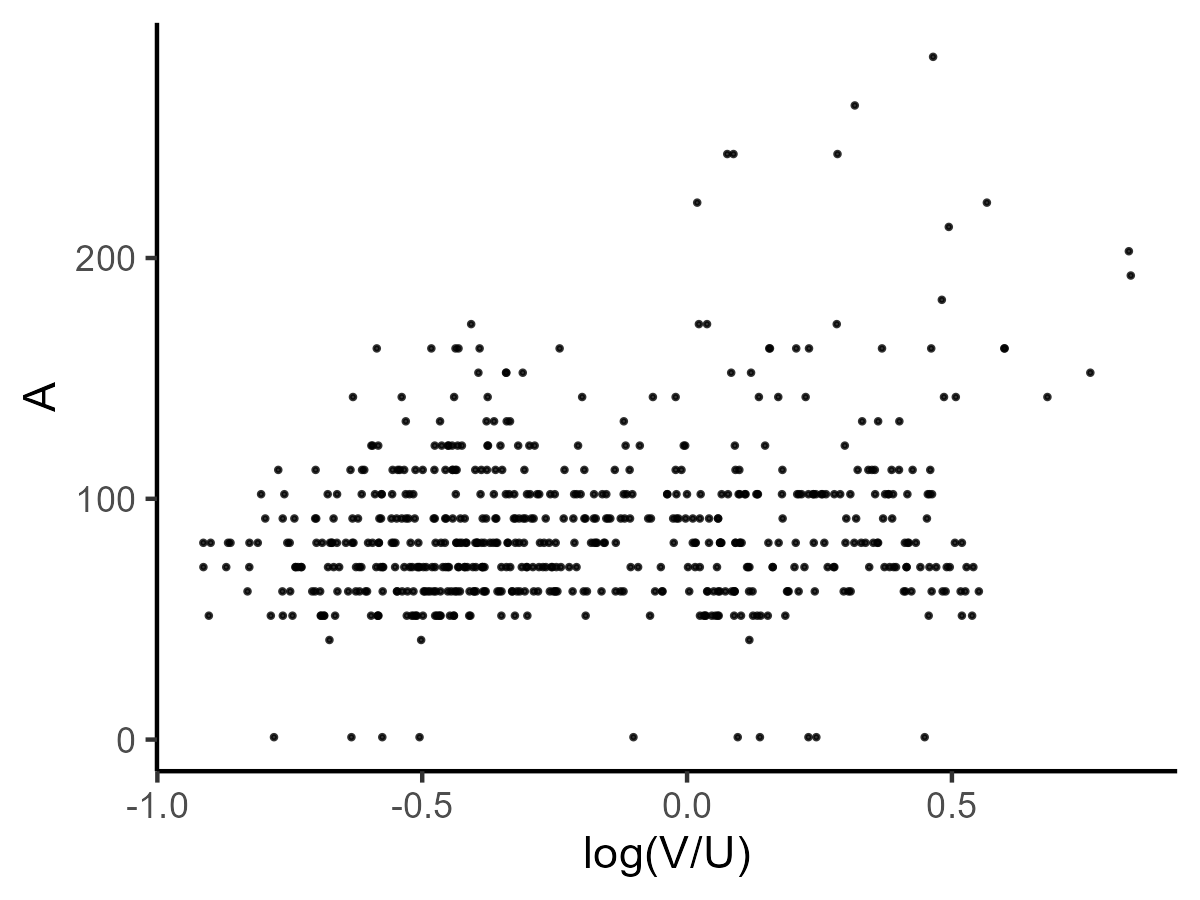
\includegraphics[width = 0.45\textwidth]
  {figuretable/efficiency_tightness_plot_month_aggregate.png}
  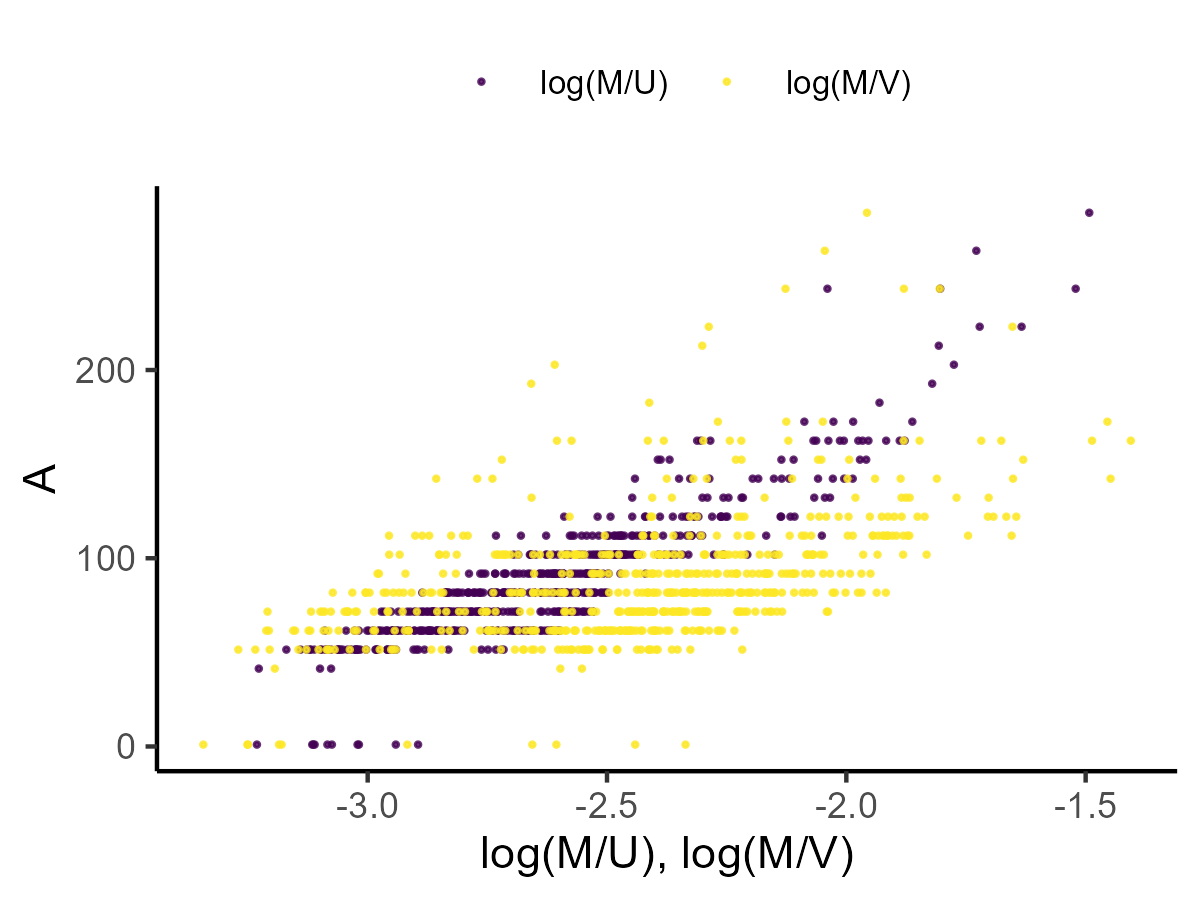
\includegraphics[width = 0.45\textwidth]
  {figuretable/job_finding_rate_efficiency_plot_month_aggregate.png}
  \end{center}
  \footnotesize
  %Note: 
\end{figure} 
\begin{itemize}
    \item Matching efficiency is correlated with tightness, i.e., inducing the endogeneity.
\end{itemize}
\end{frame}



\begin{frame}{Fact: $U,V,H$ and Tightness $V/U$ (Full-time and Part-time)}
    \begin{figure}[!ht]
  \begin{center}
  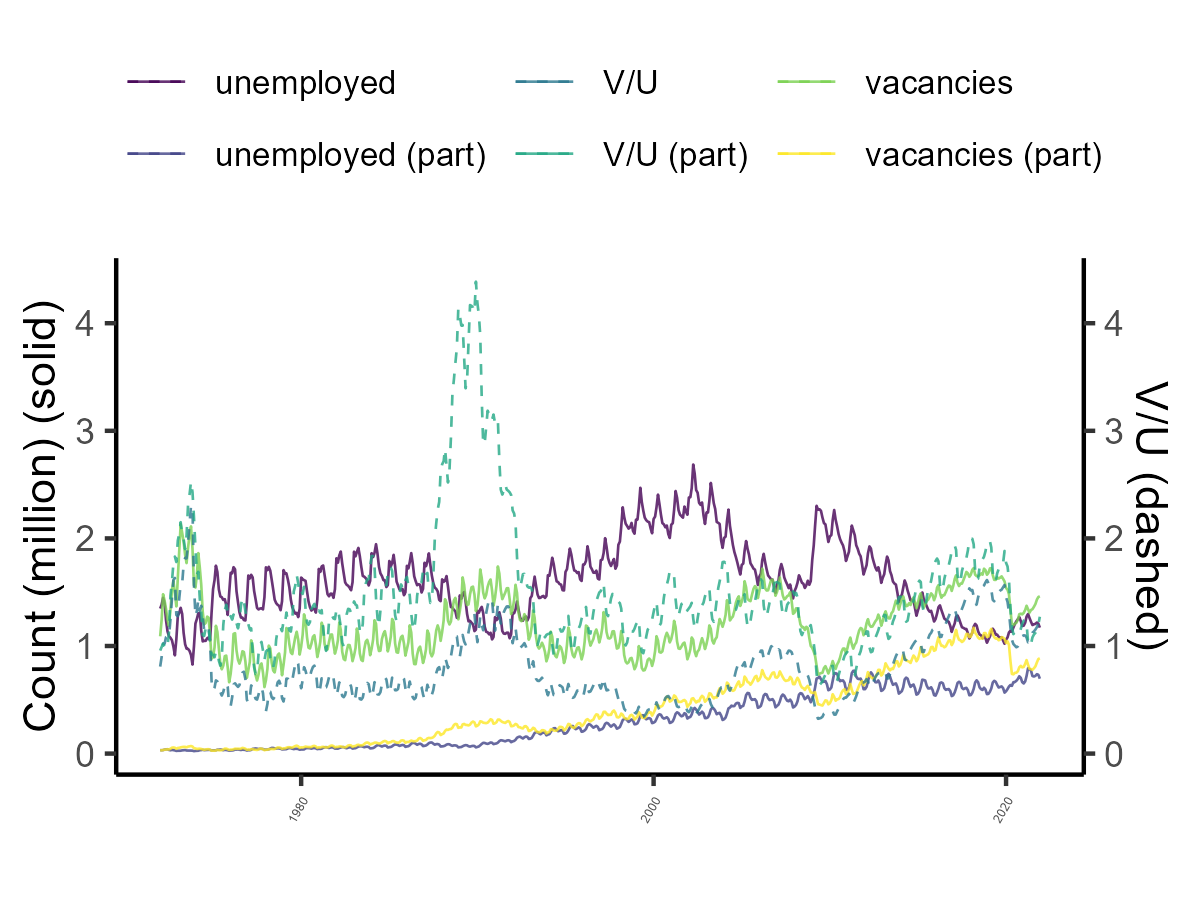
\includegraphics[width = 0.3\textwidth]
  {figuretable/unemployed_vacancy_month_full_time_part_time.png}
  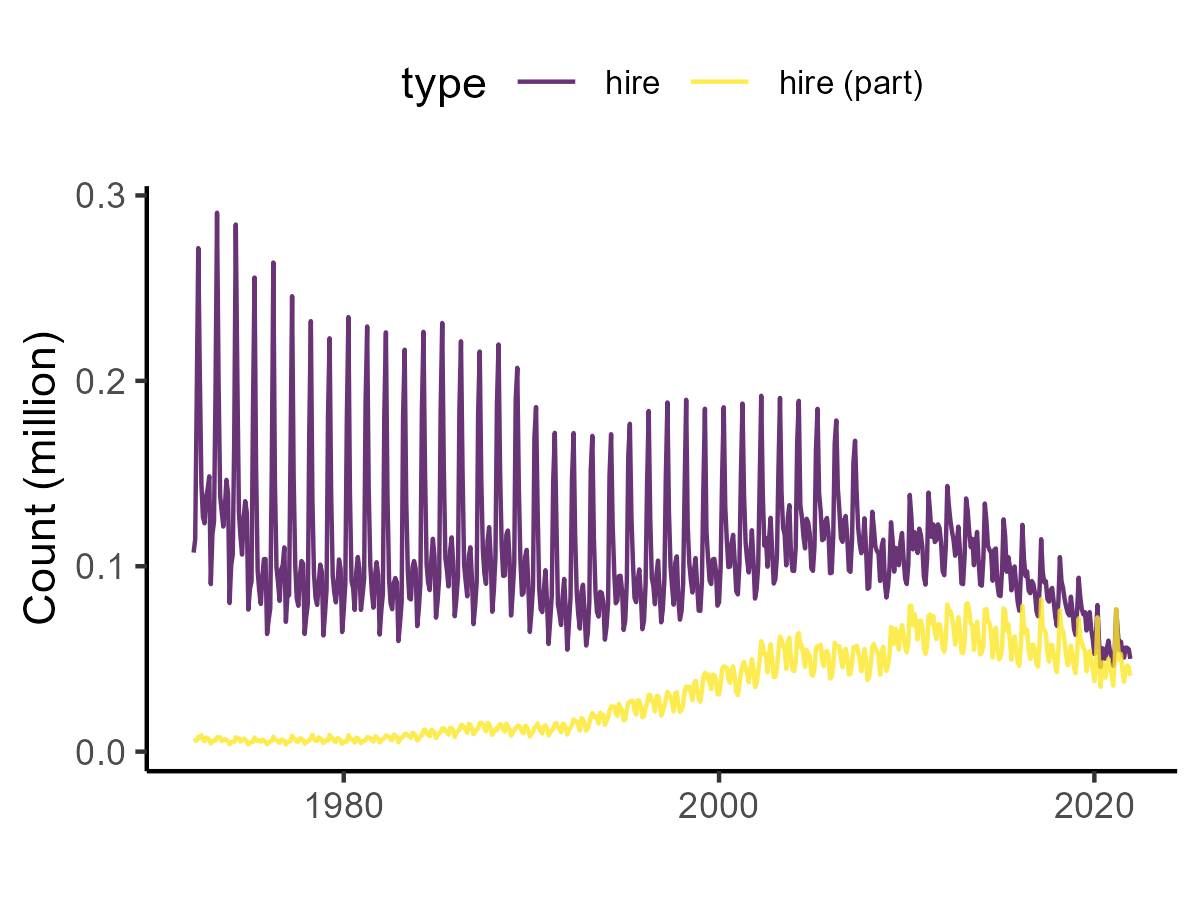
\includegraphics[width = 0.3\textwidth]
  {figuretable/hire_month_full_time_part_time.png}
  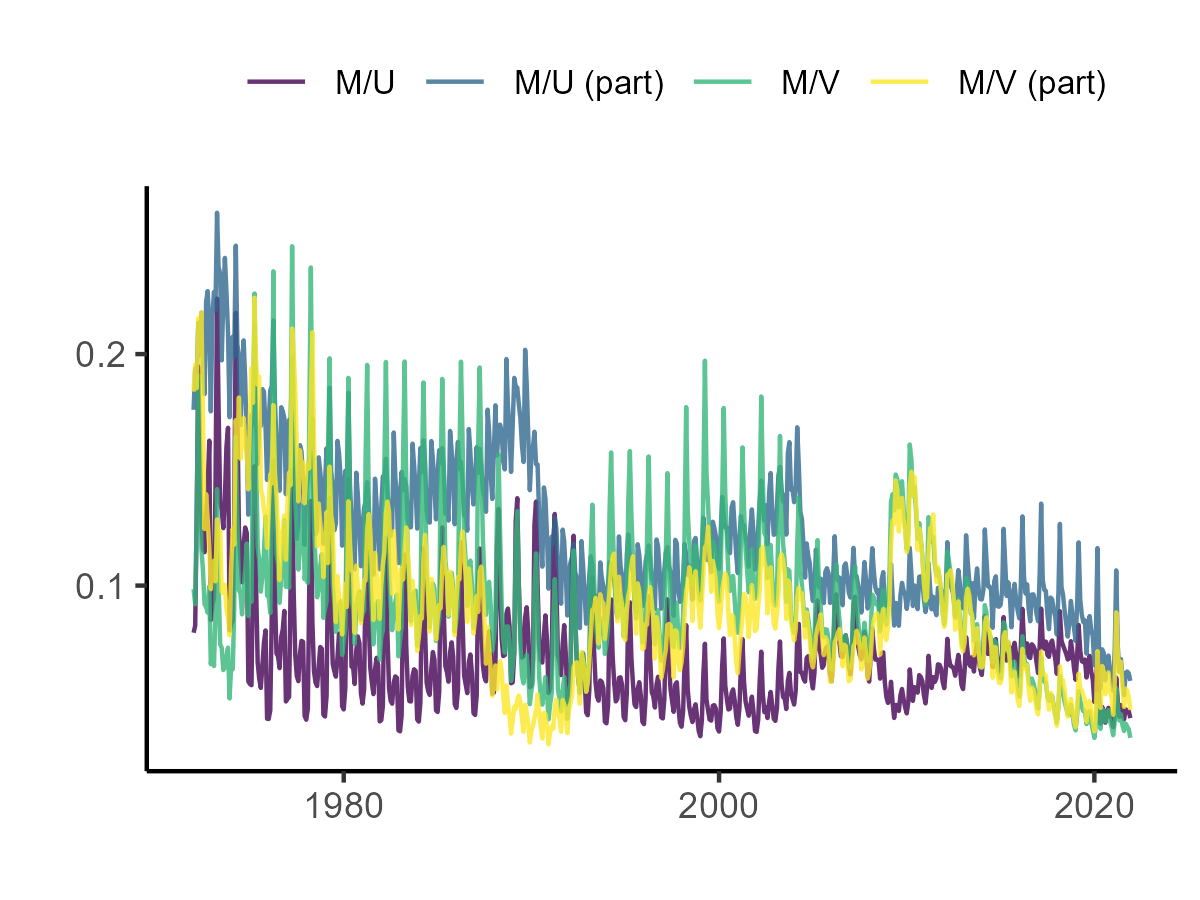
\includegraphics[width = 0.3\textwidth]
  {figuretable/job_finding_rate_worker_finding_rate_month_full_time_part_time.png}
  \end{center}
  \footnotesize
  %Note: 
\end{figure} 
\begin{itemize}
    \item Part-time hire increases steadily.
    \item Job finding rates show cyclicality.
\end{itemize}

\end{frame}

\begin{frame}{Matching Efficiency and Elasticities (Full-time and Part-time)}
    \begin{figure}[!ht]
  \begin{center}
  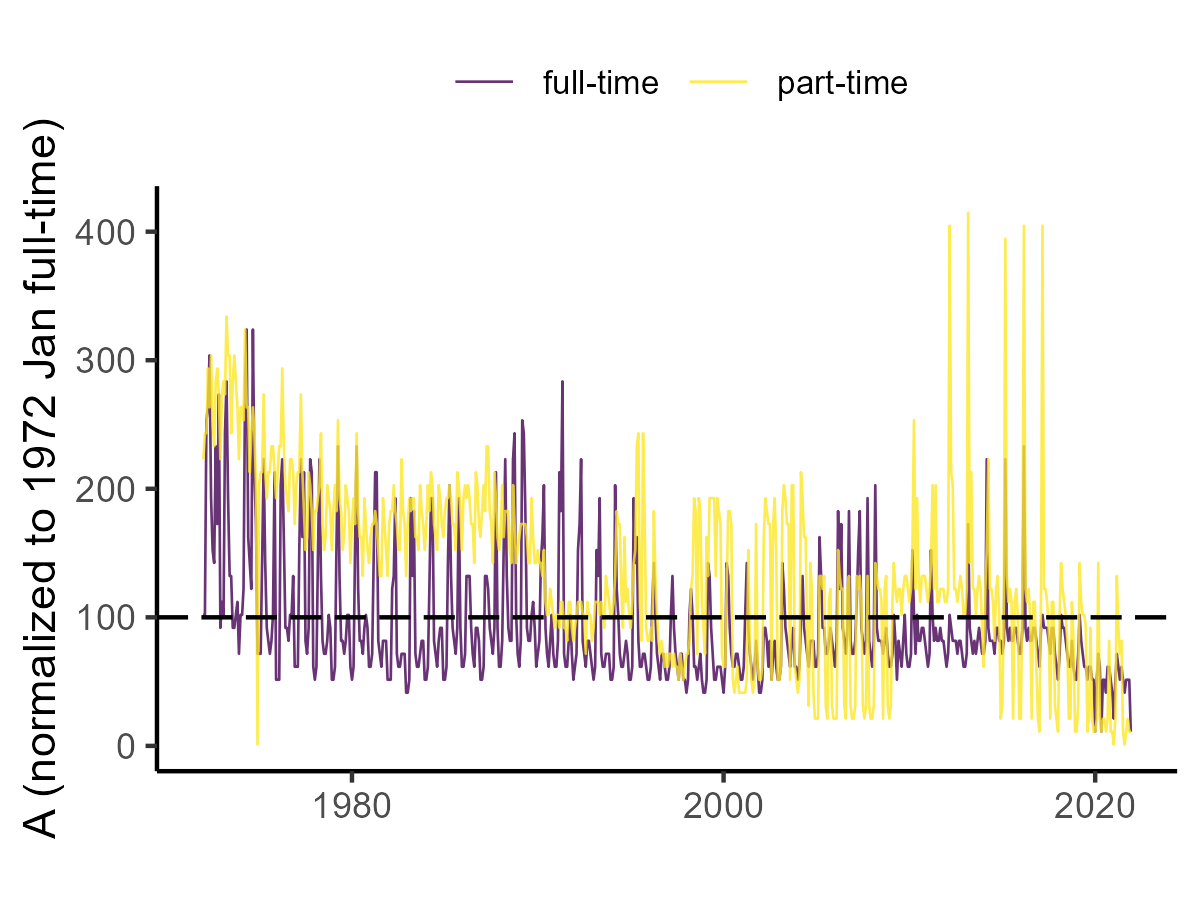
\includegraphics[width = 0.45\textwidth]
  {figuretable/matching_efficiency_month_full_time_part_time.png}
  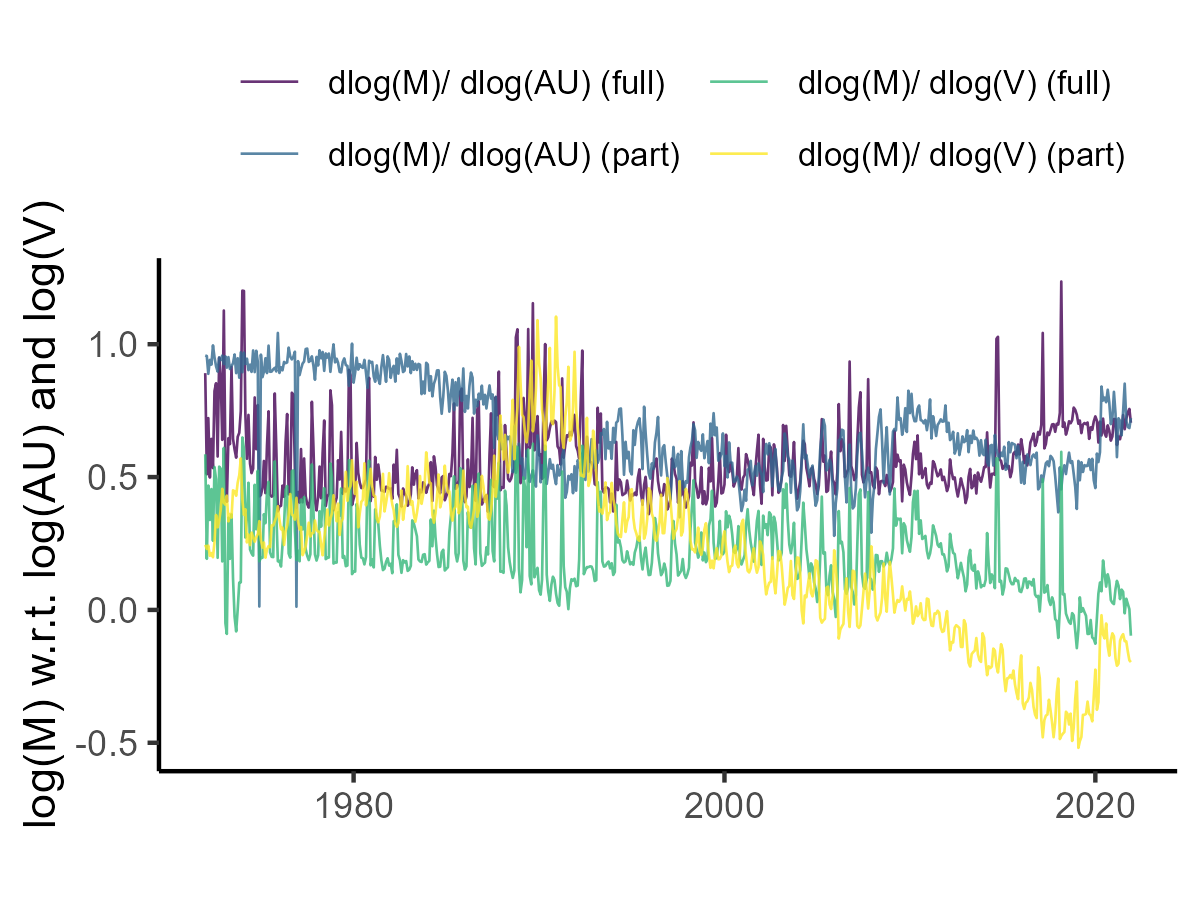
\includegraphics[width = 0.45\textwidth]
  {figuretable/elasticity_month_full_time_part_time.png}
  \end{center}
  \footnotesize
  %Note: 
\end{figure} 

\begin{itemize}
    \item Both efficiencies decrease after 2015.
    \item Matching elasticity with respect to vacancies is about 0.1 for full-time.
\end{itemize}
\end{frame}

\begin{frame}{Correlation of Efficiency and Tightness (Full-time and Part-time)}
    
\begin{figure}[!ht]
  \begin{center}
  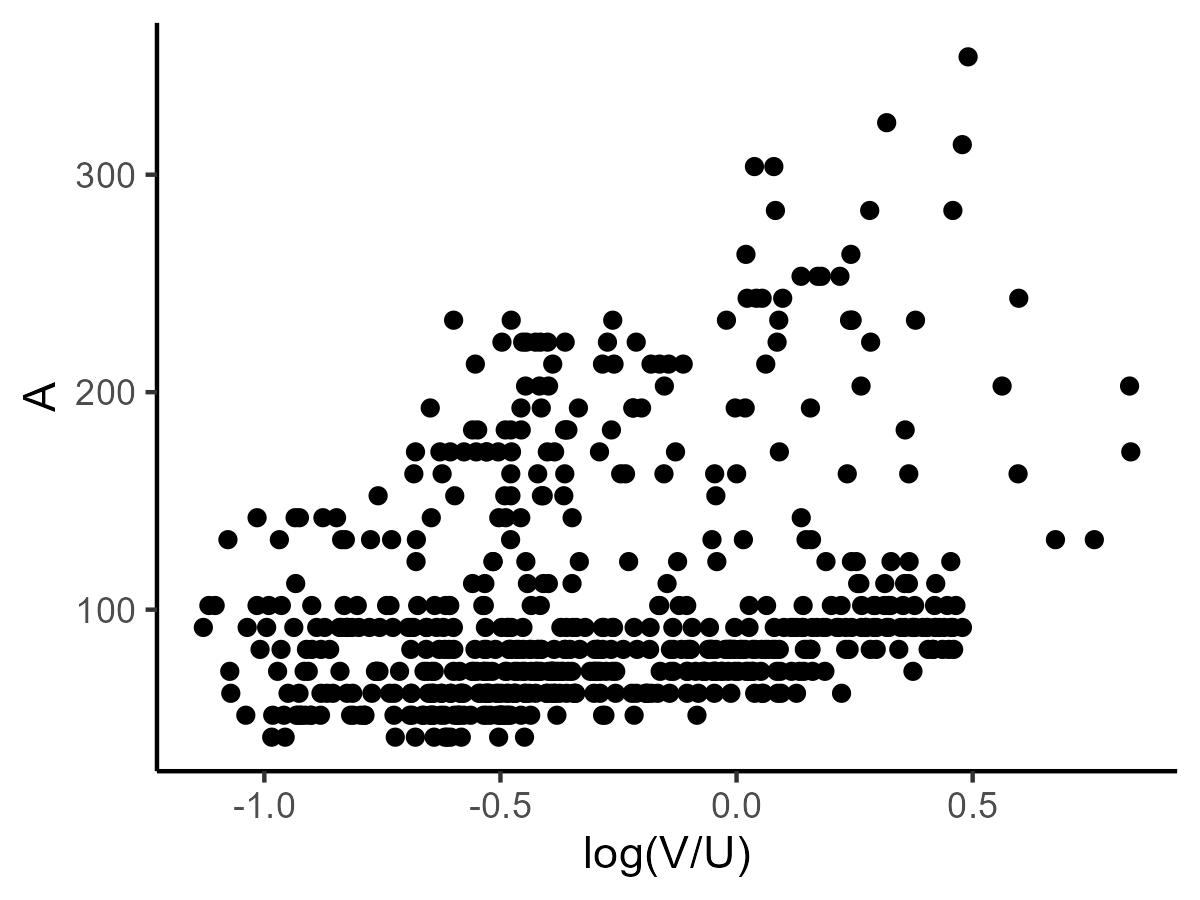
\includegraphics[width = 0.45\textwidth]
  {figuretable/efficiency_tightness_plot_month_full_time.png}
  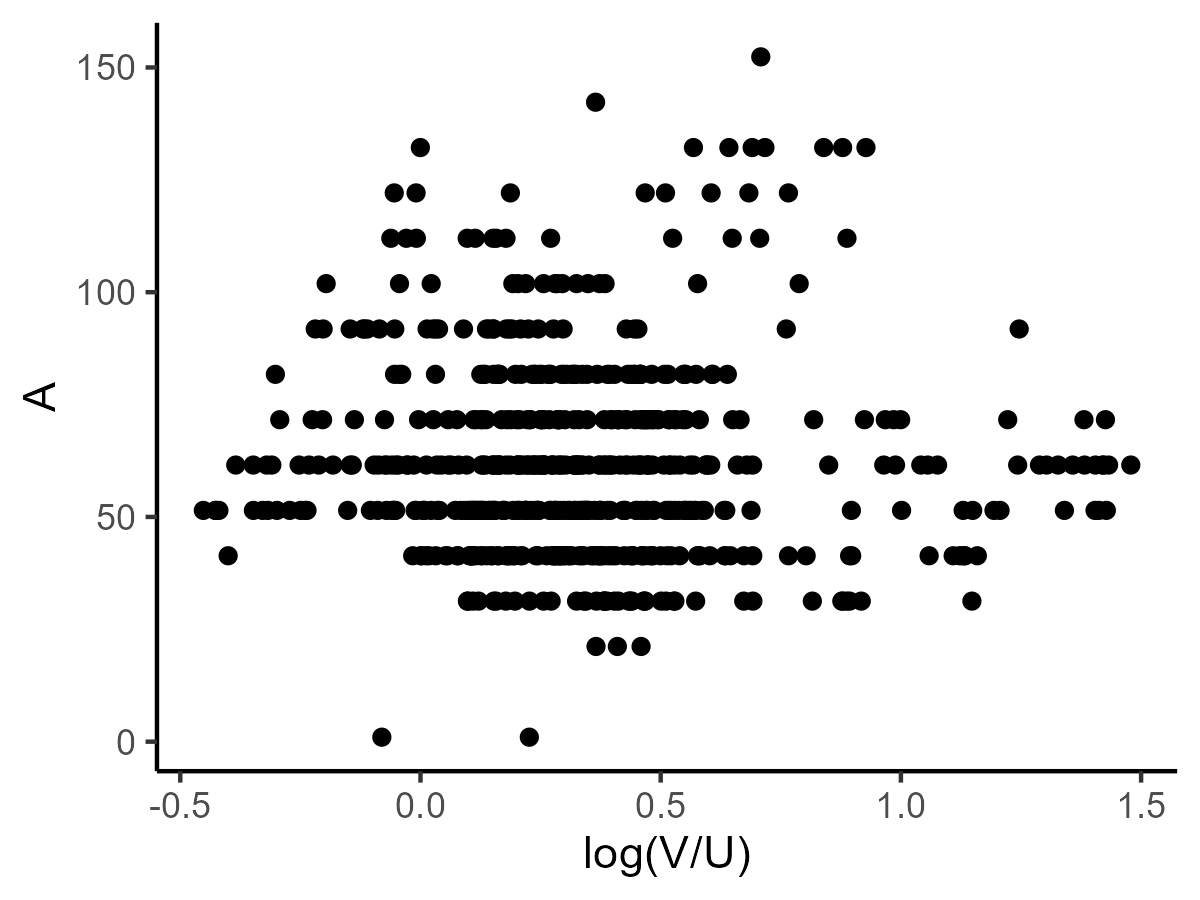
\includegraphics[width = 0.45\textwidth]
  {figuretable/efficiency_tightness_plot_month_part_time.png}
  \end{center}
  \footnotesize
  %Note: 
\end{figure} 
\begin{itemize}
    \item Full-time shows more significant correlation.
\end{itemize}
\end{frame}

\begin{frame}{Summary of long time trends}
    \begin{itemize}
        \item Matching efficiency sharply declines after 2015 by 50 \% relative to 1973.
        \begin{itemize}
            \item Driven by both full-time and part-time's efficiency declines.
        \end{itemize}
        
        \item Matching efficiency and Tightness are positively correlated.
        \begin{itemize}
            \item Full-time has a stronger correlation.
        \end{itemize}
        
    \end{itemize}
\end{frame}

\section{Empirical Results: 2012-2024}

\begin{frame}{Overview of the second empirical exercise}
    \begin{itemize}
        \item Data: Prefecture-month-level and industry-month-level data in 2012-2023.
        \item Estimate matching efficiency for each dataset.
        \begin{enumerate}
            \item All (=Full-time + Part-time)
            \item Decompose Full-time and Part-time \textcolor{blue}{[Skipped]}
        \end{enumerate}
        \item Compute nonparametric mismatch index across prefectures and industries
        \begin{enumerate}
            \item All (=Full-time + Part-time)
            \item Decompose Full-time and Part-time \textcolor{blue}{[Skipped]}
        \end{enumerate}
    \end{itemize}
\end{frame}

\begin{frame}{Matching Efficiency: Tohoku and Kanto}
\begin{figure}[!ht]
  \begin{center}

  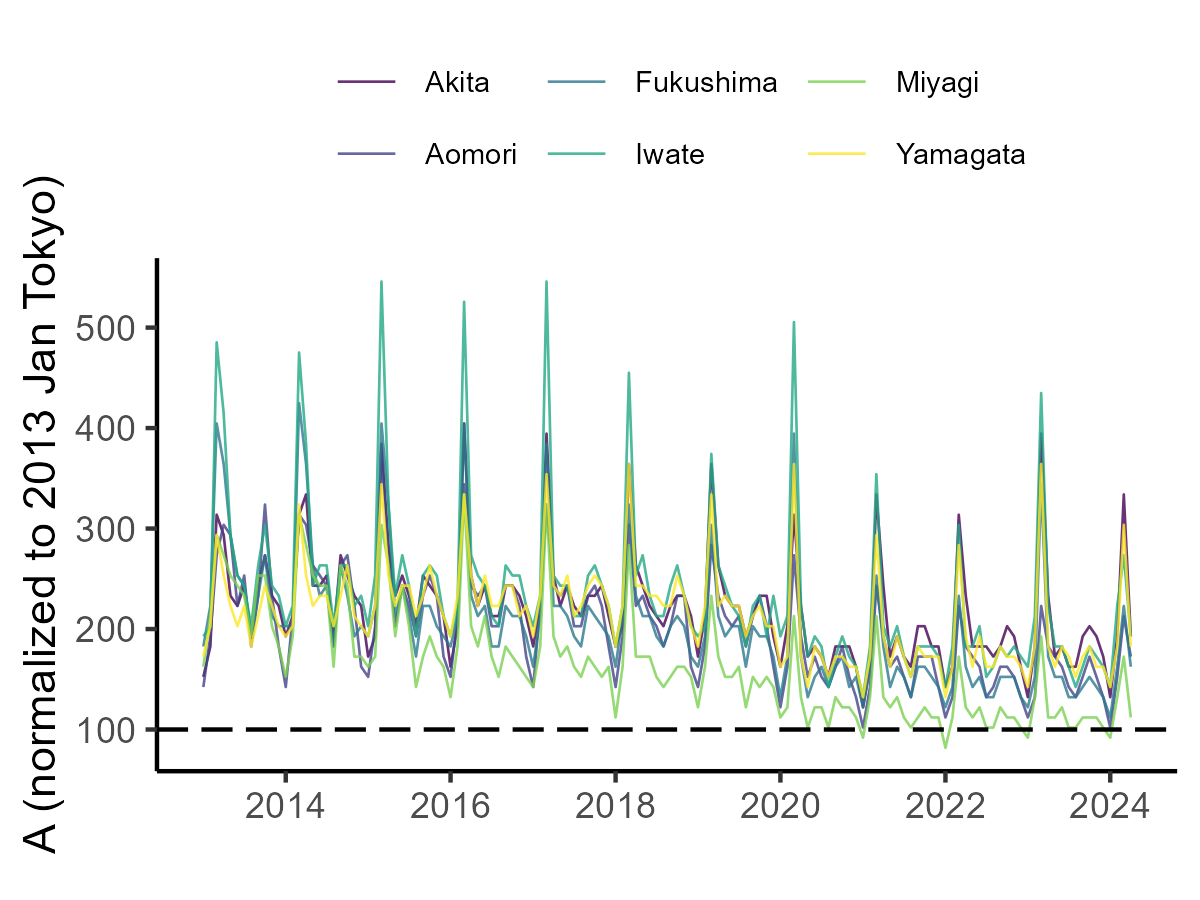
\includegraphics[width = 0.45\textwidth]
  {figuretable/matching_efficiency_month_aggregate_tohoku.png}
  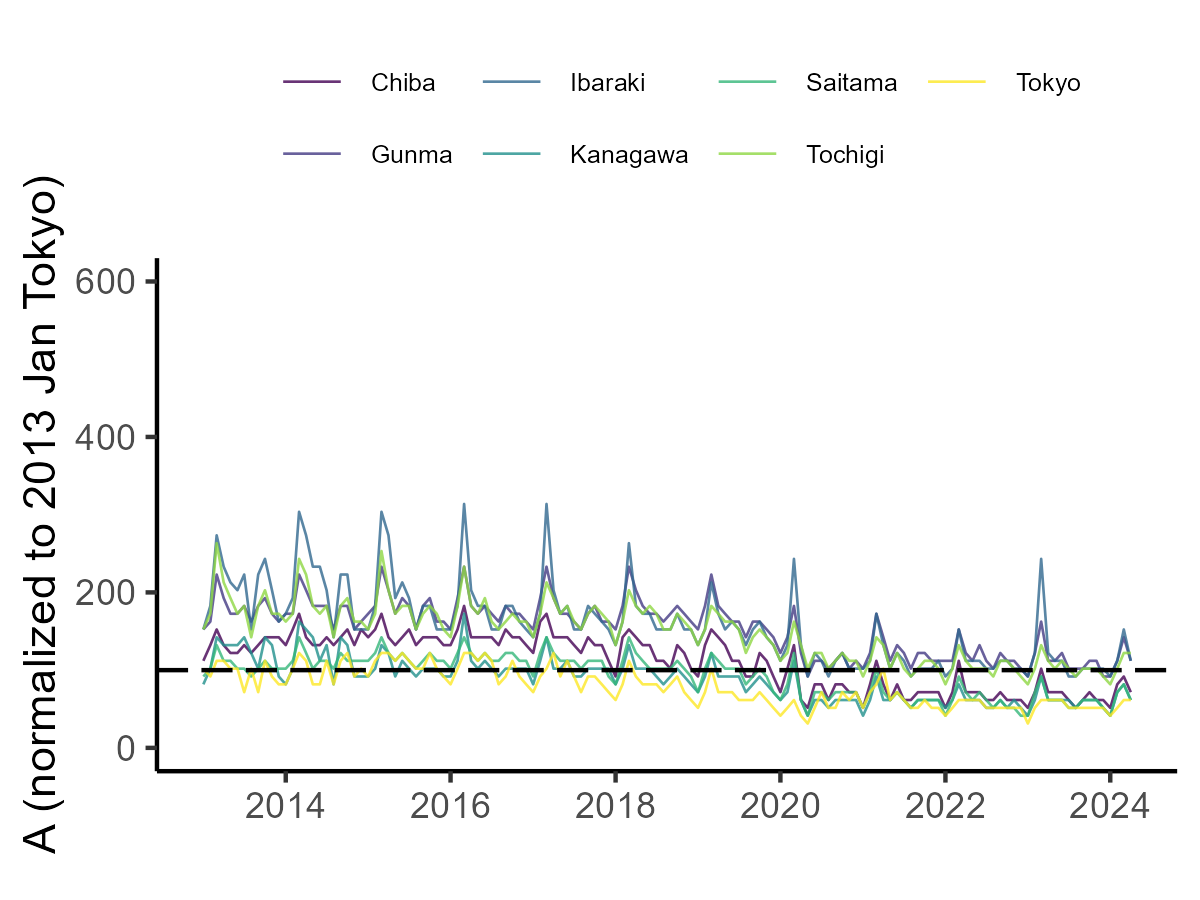
\includegraphics[width = 0.45\textwidth]
  {figuretable/matching_efficiency_month_aggregate_kanto.png}
  % \subfloat[Chubu]{\includegraphics[width = 0.45\textwidth]
  % {figuretable/matching_efficiency_month_aggregate_chubu.png}}
  % \\
  % \subfloat[Kansai]{\includegraphics[width = 0.45\textwidth]
  % {figuretable/matching_efficiency_month_aggregate_kansai.png}}
  % \subfloat[Chugoku]{\includegraphics[width = 0.45\textwidth]
  % {figuretable/matching_efficiency_month_aggregate_chugoku.png}}\\
  % \subfloat[Shikoku]{\includegraphics[width = 0.45\textwidth]
  % {figuretable/matching_efficiency_month_aggregate_shikoku.png}}
  % \subfloat[Kyusyu, Okinawa]{\includegraphics[width = 0.45\textwidth]
  % {figuretable/matching_efficiency_month_aggregate_kyushu.png}}
  % \caption{Month-level aggregate results 2012-2024}
  % \label{fg:month_part_and_full_time_matching_efficiency_prefecture_results} 
  \end{center}
  \footnotesize
  %Note: 
\end{figure} 
\begin{itemize}
    \item Tohoku area is twice more efficient than Tokyo area.
\end{itemize}
\end{frame}

\begin{frame}{Matching Elasticities: Tohoku and Kanto}
\begin{figure}[!ht]
  \begin{center}
  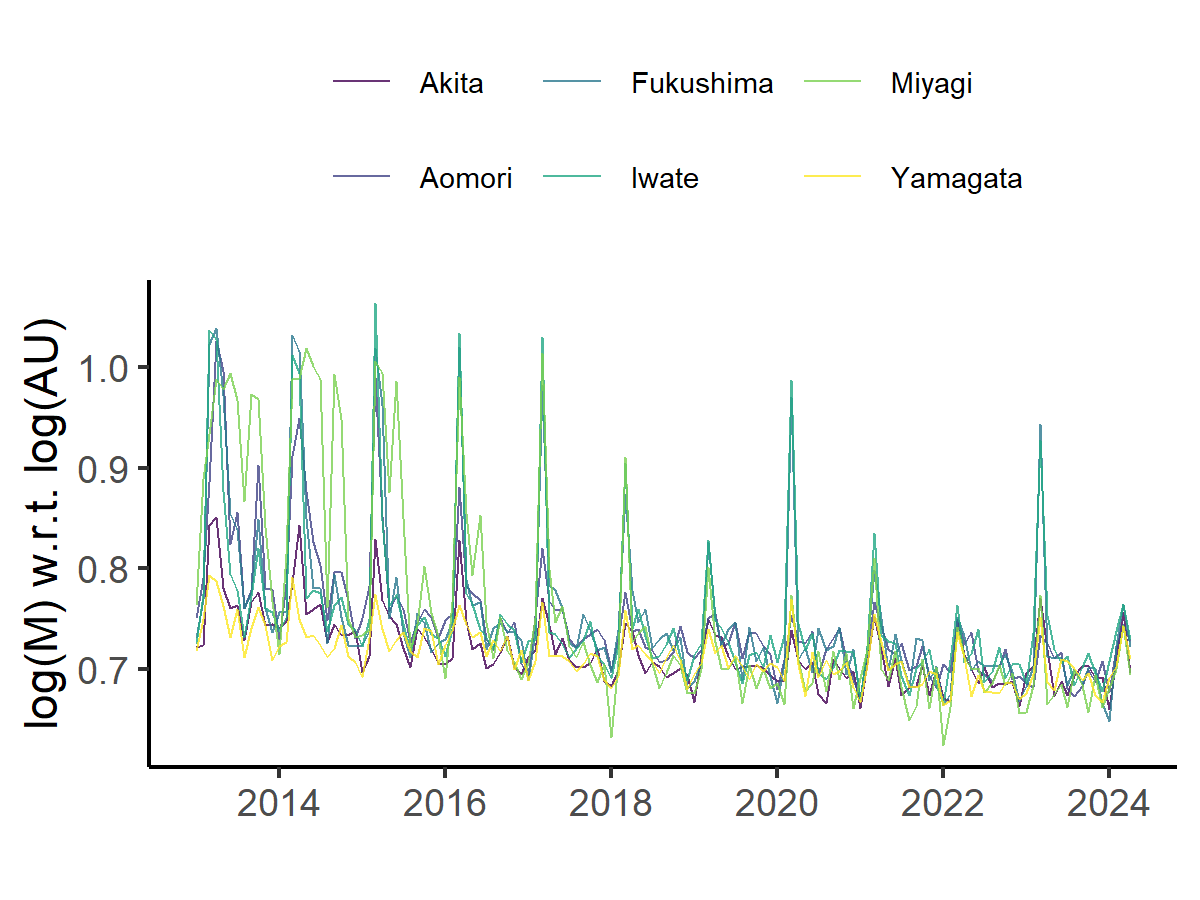
\includegraphics[width = 0.45\textwidth]
  {figuretable/elasticity_unemployed_month_aggregate_tohoku.png}
  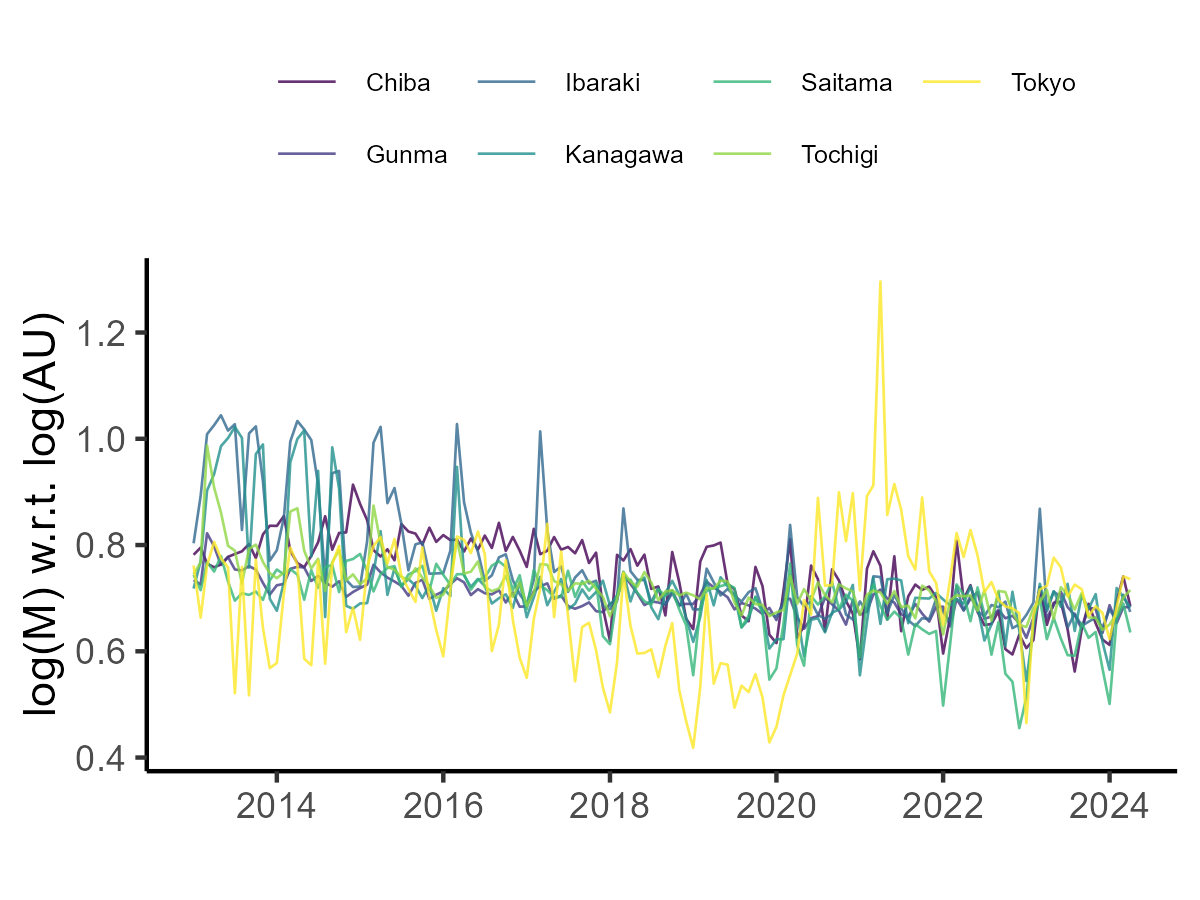
\includegraphics[width = 0.45\textwidth]
  {figuretable/elasticity_unemployed_month_aggregate_kanto.png}
  % \subfloat[Chubu]{\includegraphics[width = 0.45\textwidth]
  % {figuretable/elasticity_unemployed_month_aggregate_chubu.png}}
  % \\
  % \subfloat[Kansai]{\includegraphics[width = 0.45\textwidth]
  % {figuretable/elasticity_unemployed_month_aggregate_kansai.png}}
  % \subfloat[Chugoku]{\includegraphics[width = 0.45\textwidth]
  % {figuretable/elasticity_unemployed_month_aggregate_chugoku.png}}\\
  % \subfloat[Shikoku]{\includegraphics[width = 0.45\textwidth]
  % {figuretable/elasticity_unemployed_month_aggregate_shikoku.png}}
  % \subfloat[Kyusyu, Okinawa]{\includegraphics[width = 0.45\textwidth]
  % {figuretable/elasticity_unemployed_month_aggregate_kyushu.png}}
  % \caption{Month-level aggregate results 2012-2024}
  % \label{fg:month_part_and_full_time_elasticity_unemployed_month_aggregate_prefecture_results} 
  \end{center}
  \footnotesize
  %Note: 
\end{figure} 
\begin{itemize}
    \item Tohoku area shows 0.7-0.8 , Tokyo area shows 0.6-0.7.
\end{itemize}
\end{frame}

\begin{frame}{Matching Efficiency: Clerical and Agriculture\&Fishery}
\begin{figure}[!ht]
  \begin{center}
  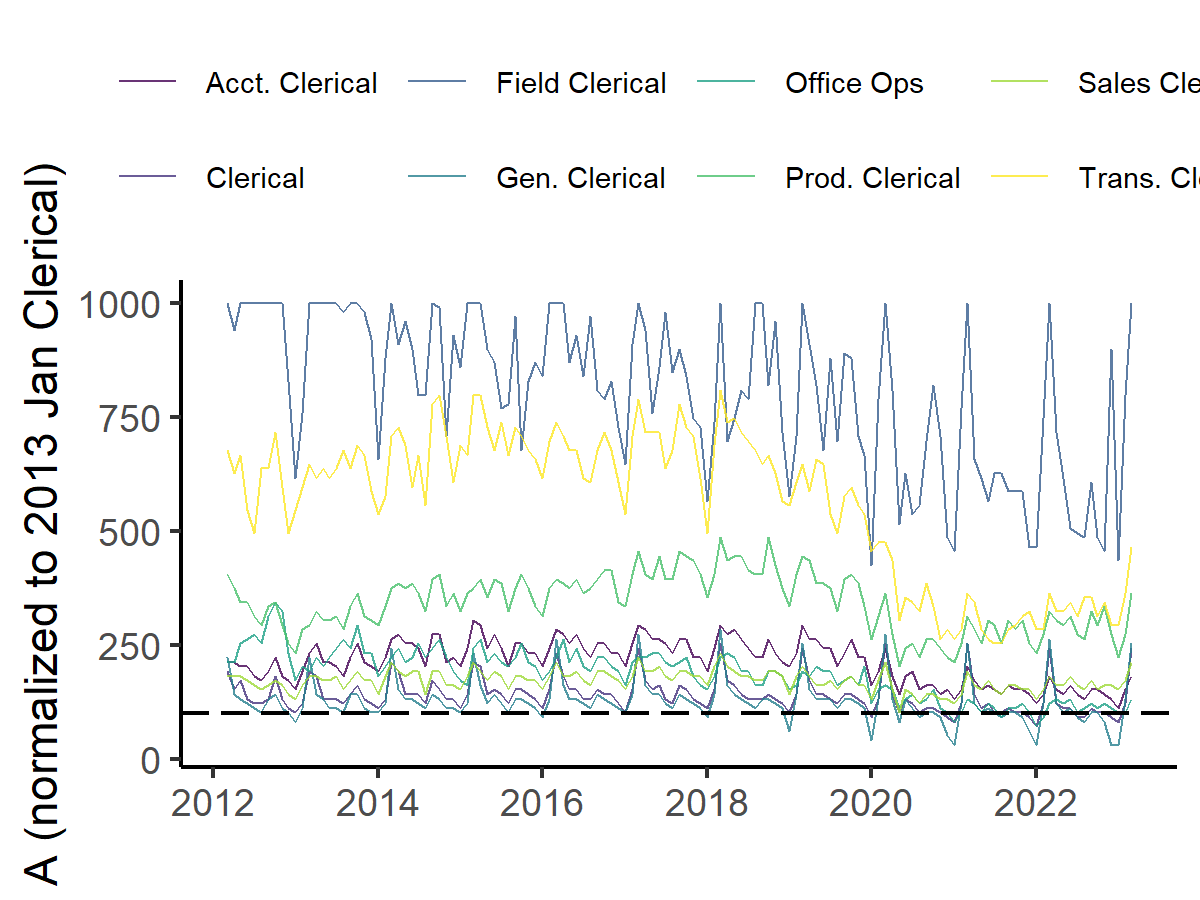
\includegraphics[width = 0.45\textwidth]
  {figuretable/matching_efficiency_month_aggregate_clerical.png}
  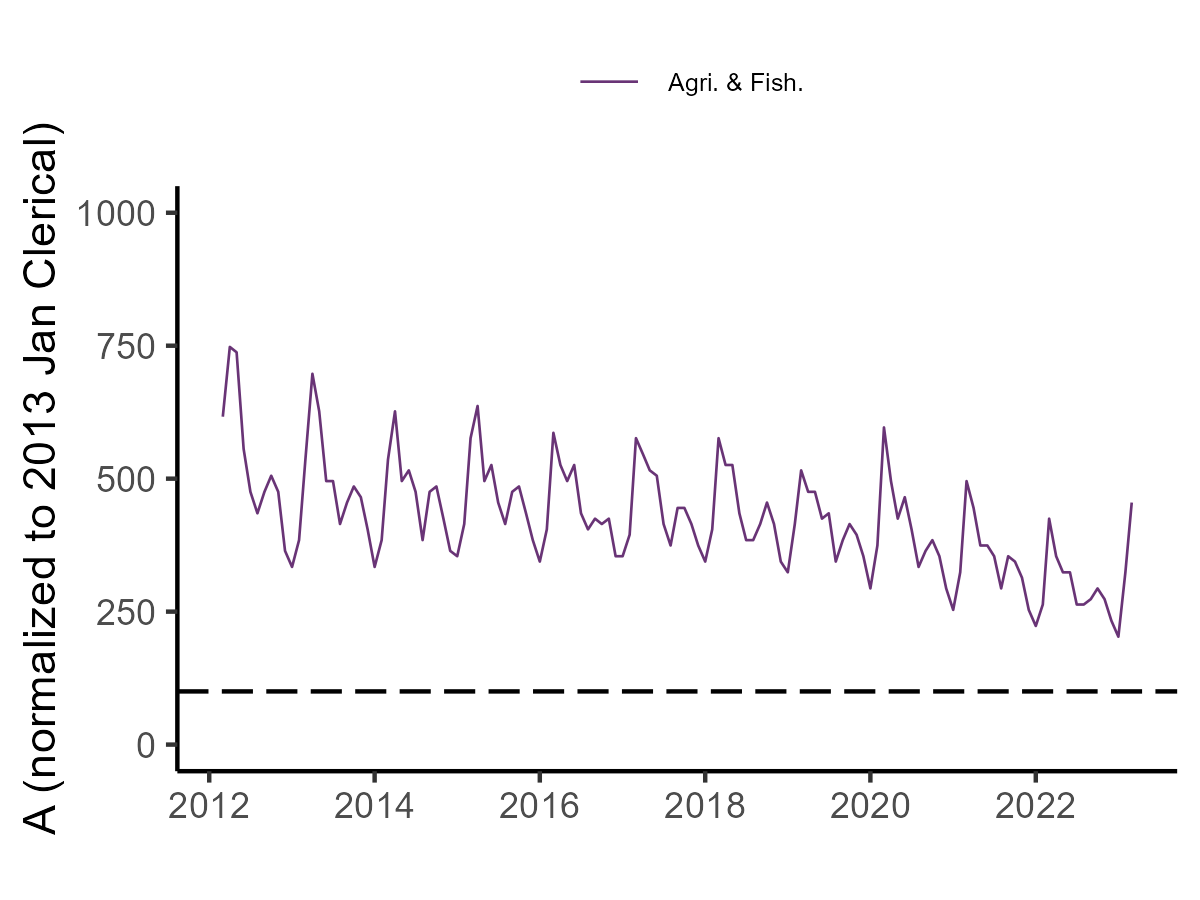
\includegraphics[width = 0.45\textwidth]
  {figuretable/matching_efficiency_month_aggregate_agriculture_forestry_and_fishing.png}
  \end{center}
  \footnotesize
  %Note: 
\end{figure} 
    \begin{itemize}
        \item Clerical jobs are heterogeneous within the industries.
        \item Agriculture and Fishery industries show higher efficiency than clerical.
    \end{itemize}
\end{frame}

% \begin{frame}{Matching Elasticity: Clerical and Agriculture\&Fishery}
%     \begin{figure}[!ht]
%   \begin{center}
%   \includegraphics[width = 0.45\textwidth]
%   {figuretable/elasticity_unemployed_month_aggregate_clerical.png}
%   \includegraphics[width = 0.45\textwidth]
%   {figuretable/elasticity_unemployed_month_aggregate_agriculture_forestry_and_fishing.png}
%   \end{center}
%   \footnotesize
%   %Note: 
% \end{figure} 
%     \begin{itemize}
%         \item Clerical [TBA]
%     \end{itemize}
% \end{frame}

\begin{frame}{Mismatch across prefectures and job categories}
\begin{figure}[!ht]
  \begin{center}

  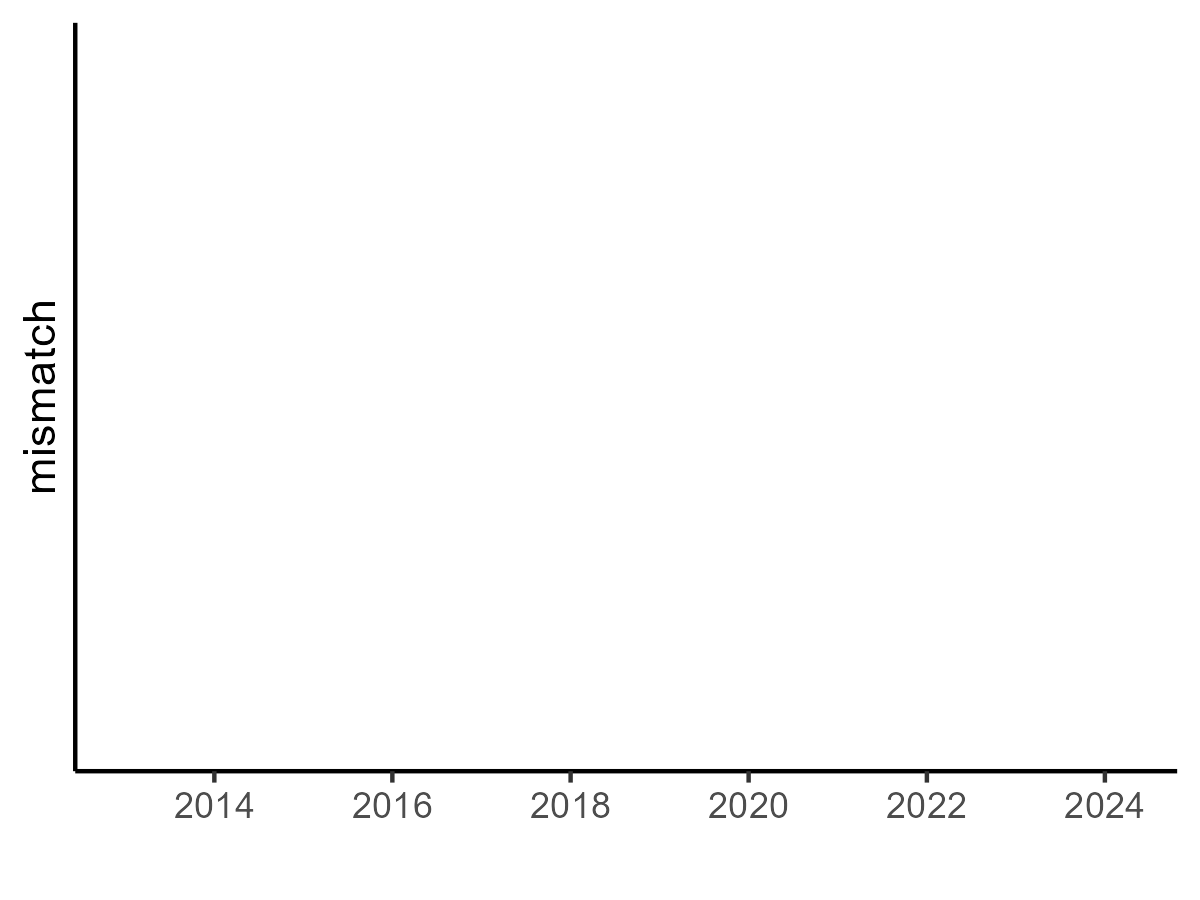
\includegraphics[width = 0.45\textwidth]
  {figuretable/mismatch_part_and_full_time_monthly_prefecture.png}
  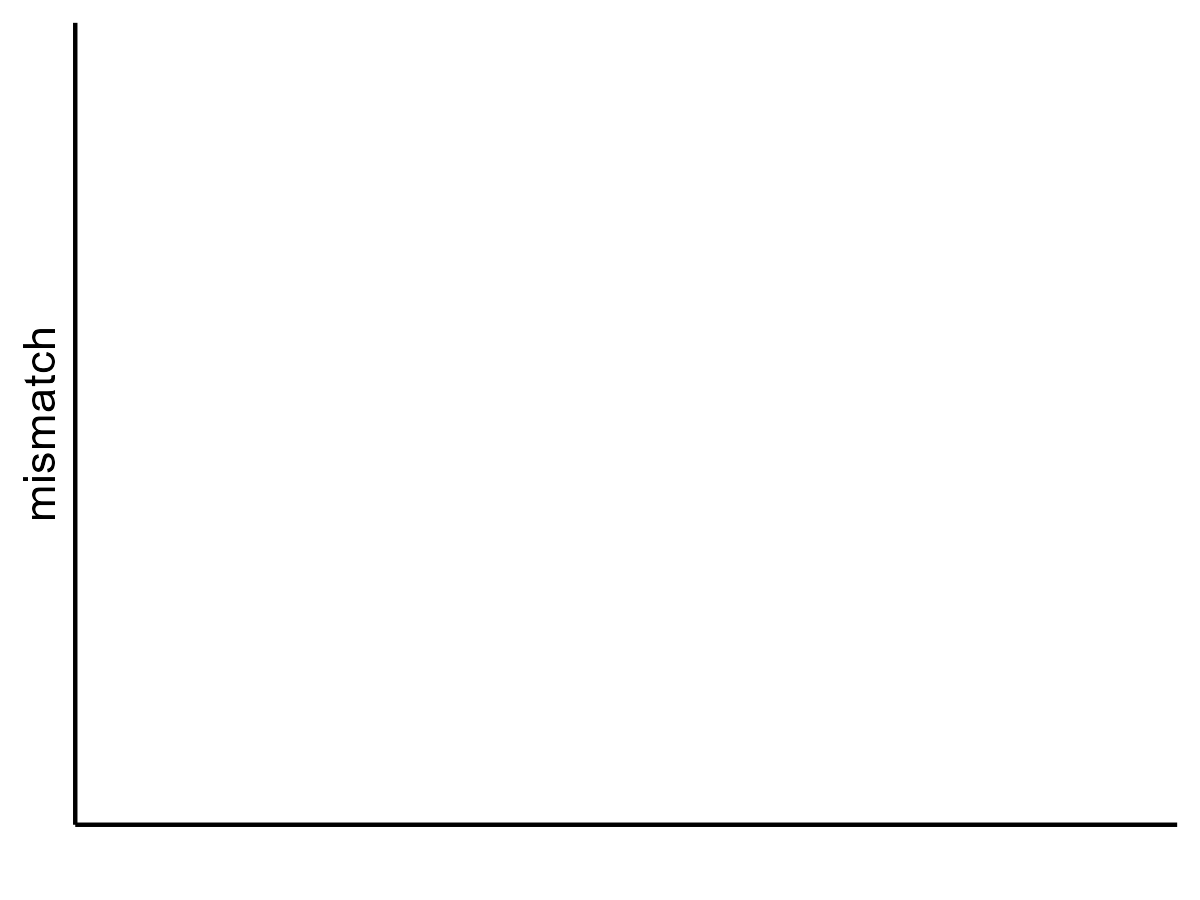
\includegraphics[width = 0.45\textwidth]
  {figuretable/mismatch_part_and_full_time_monthly_job_category.png}
  \end{center}
  \footnotesize
  %Note: 
\end{figure} 
\begin{itemize}
    \item Mismatch across prefectures increases to around 0.1.
    \item Mismatch across job categories increases to 0.3.
\end{itemize}

\end{frame}


\begin{frame}{Summary of short time trends}
    \begin{itemize}
        \item Matching efficiency \textbf{decreases}.
        \item Mismatch across prefectures increases to 0.1.
        \item Mismatch across industries increases to 0.3.
        \begin{itemize}
            \item Previous studies (0.2) are underestimated.
        \end{itemize}
    \end{itemize}
\end{frame}

\begin{frame}{Conclusion and Future work}
    \begin{itemize}
      \item Contributions and Findings
      \begin{itemize}
          \item Examine nonparametric approach and its finite sample performance.
          \item Compute nonparametric mismatch index.
          \item Matching efficiency decreases and is driven by both full-time and part-time.
          \item Mismatch increases in particular across job categories.
      \end{itemize}
      \item Future work
      \begin{itemize}
          \item Examine bias of the Cobb Douglas results.
          \item Interesting counterfactual for a social planner.
          \item Endogeneity issues (Imbens and Newey (2009)).
      \end{itemize}
    \end{itemize}
\end{frame}

\end{document}